%%%%%%%%%%%%%%%%%%%%%%%%%%%%%%%%%%%%%%%%%%%%%%%%%%%%%%%%%%%%%%%%%%%%%%
% Overleaf (WriteLaTeX) Example: Molecular Chemistry Presentation
%
% Source: http://www.overleaf.com
%
% In these slides we show how Overleaf can be used with standard 
% chemistry packages to easily create professional presentations.
% 
% Feel free to distribute this example, but please keep the referral
% to overleaf.com
% 
%%%%%%%%%%%%%%%%%%%%%%%%%%%%%%%%%%%%%%%%%%%%%%%%%%%%%%%%%%%%%%%%%%%%%%

\documentclass{beamer}

\mode<presentation>
{
  \usetheme{Madrid}       % or try default, Darmstadt, Warsaw, ...
  \usecolortheme{default} % or try albatross, beaver, crane, ...
  \usefonttheme{default}    % or try default, structurebold, ...
  \setbeamertemplate{navigation symbols}{}
  \setbeamertemplate{caption}[numbered]
} 

\usepackage[english]{babel}
\usepackage[utf8x]{inputenc}
\usepackage{graphicx}
\usepackage{hyperref}
  \hypersetup{colorlinks=true}
  \hypersetup{urlcolor=blue}
  \hypersetup{linkcolor = .}
\usepackage{xcolor}
\usepackage{siunitx}
  \sisetup{separate-uncertainty = true}
\usepackage{physics}
\usepackage[font=small,labelfont=bf,justification=centering]{caption}
\usepackage{subcaption}
\usepackage[en-GB]{datetime2}
\usepackage{overpic}
\usepackage{feynmp}
\DeclareGraphicsRule{*}{mps}{*}{}
\usepackage{scalerel}
\newcommand{\mylbrace}[2]{\vspace{#2pt}\hspace{6pt}\scaleleftright[\dimexpr5pt+#1\dimexpr0.06pt]{\lbrace}{\rule[\dimexpr2pt-#1\dimexpr0.5pt]{-4pt}{#1pt}}{.}}
\newcommand{\myrbrace}[2]{\vspace{#2pt}\scaleleftright[\dimexpr5pt+#1\dimexpr0.06pt]{.}{\rule[\dimexpr2pt-#1\dimexpr0.5pt]{-4pt}{#1pt}}{\rbrace}\hspace{6pt}}
\usepackage{ulem} % Line across text
\newcommand{\white}[1]{{\textcolor{white}{#1}}} % White text

% Here's where the presentation starts, with the info for the title slide
\title[$K^+K^-\pi^+\pi^-$]{\texorpdfstring{$D\to K^+K^-\pi^+\pi^-$}{K+K-pi+pi-} strong phase analysis and introduction to TORCH analysis}

\author{Martin Tat}
\institute{Oxford LHCb}
\date{29th January 2024}

\titlegraphic{
\includegraphics[height = 2cm]{lhcb.jpg}\hspace{1cm}~%
              
\includegraphics[height = 2cm]{OxfordLogo.pdf}\hspace{1cm}~%
              
\includegraphics[height = 2cm]{bes3.jpg}}

\begin{document}

\begin{frame}
  \titlepage
\end{frame}

% These three lines create an automatically generated table of contents.
%\begin{frame}{Outline}
%  \tableofcontents
%\end{frame}

\section{Introduction}

\begin{frame}{Brief recap of BESIII analysis}
  \begin{center}
    \Large{What I presented in December:}
  \end{center}
  \vspace{0.1cm}
  \begin{itemize}
    \setlength\itemsep{0.7em}
    \item{BESIII measurement of $c_i$ and $s_i$ in $D^0\to K^+K^-\pi^+\pi^-$}
    \item{Asymmetric uncertainties on $s_i$ using Plugin method}
    \item{New review committee, no showstoppers so far}
  \end{itemize}
  \begin{figure}
    \centering
    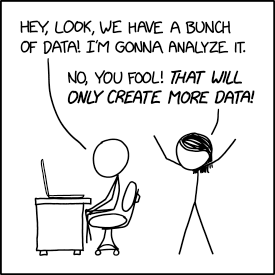
\includegraphics[width = 0.3\textwidth]{Plots/XKCD_Data_Trap.png}
  \end{figure}
  \begin{center}
    \Large{While in review, more BESIII has become available!}
  \end{center}
\end{frame}

\begin{frame}{Status of BESIII data taking}
  \begin{center}
    \Large{BESIII will collect $\SI{20}{\per\femto\barn}$ at $\psi(3770)$:}
  \end{center}
  \vspace{0.1cm}
  \begin{enumerate}
    \setlength\itemsep{0.7em}
    \item{2010-2011: $\SI{2.93}{\per\femto\barn}\quad\leftarrow\quad$ Measurement of $F_+$}
    \item{2021-2022: $\SI{4.995}{\per\femto\barn}\quad\leftarrow\quad$ Previous presentation}
    \item{2022-2023: $\SI{8.157}{\per\femto\barn}\quad\leftarrow\quad$ New stuff!}
    \item{2023-2024: Data taking ongoing}
  \end{enumerate}
  \begin{figure}
    \centering
    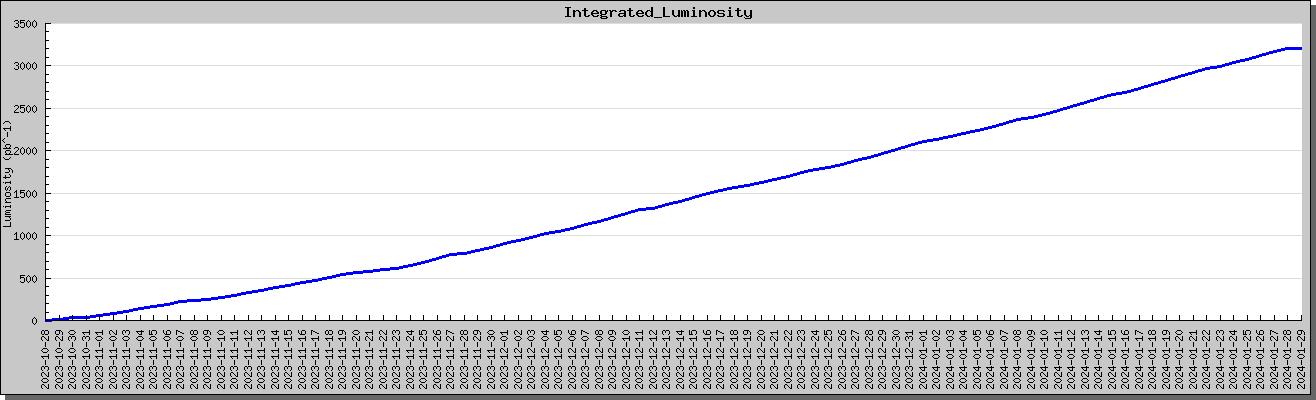
\includegraphics[width = 1.0\textwidth]{Plots/BESIII_Luminosity.png}
  \end{figure}
\end{frame}

\section{Preliminary look at new $\psi(3770)$ data}

\begin{frame}{Cross check of $D^0\to K^+K^-\pi^+\pi^-$ ST yield}
  \begin{center}
    {\large Check that ST yield agrees with integrated luminosity}
  \end{center}
  \vspace{0.1cm}
  \begin{itemize}
    \item{ST yields used for normalisation}
    \item{Expect a factor $2$ increase}
  \end{itemize}
  \begin{figure}
    \centering
    \begin{subfigure}{0.4\textwidth}
      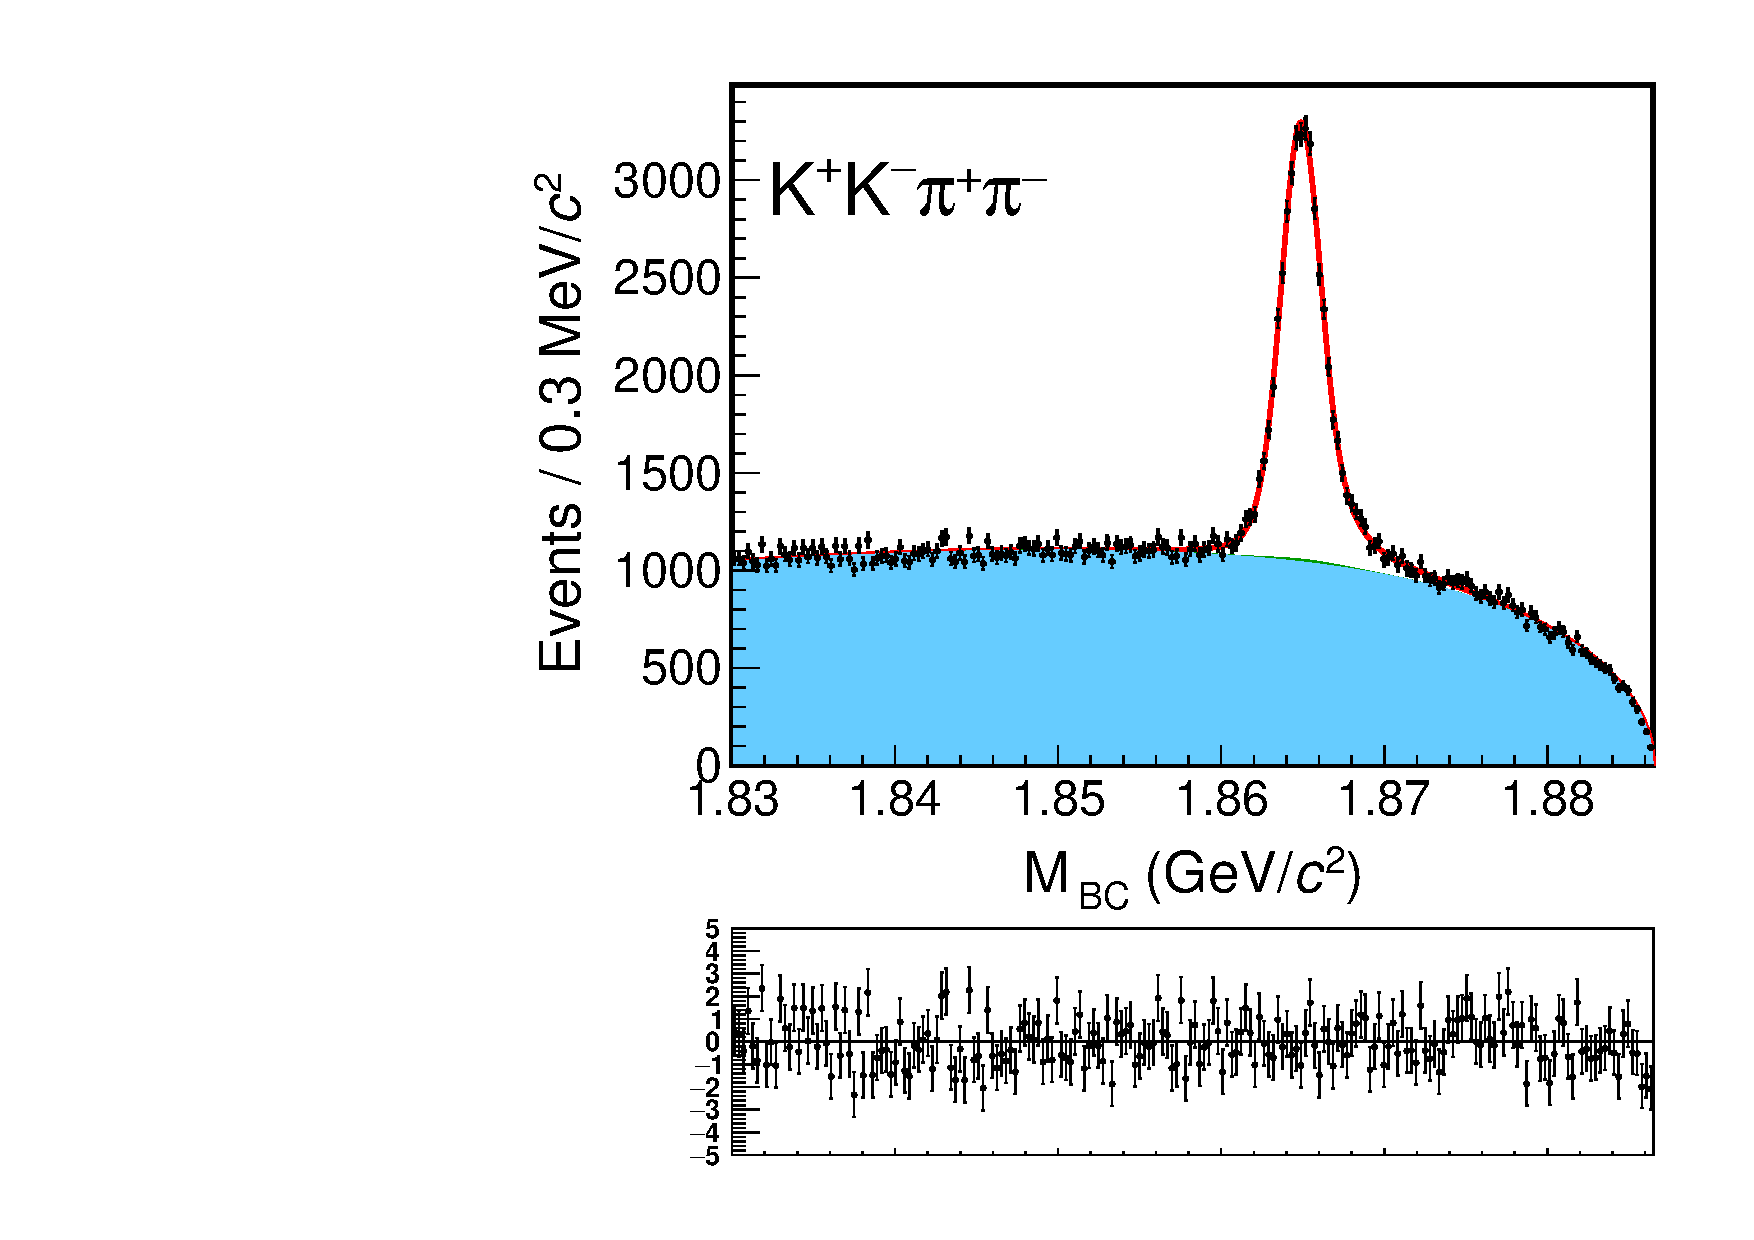
\includegraphics[width = 1.0\textwidth]{Plots/KKpipi_SingleTag_MBC_Plot_8invfb.pdf}
      \caption{$N = 29227 \pm 268$}
    \end{subfigure}%
    \hspace{1cm}
    \begin{subfigure}{0.4\textwidth}
      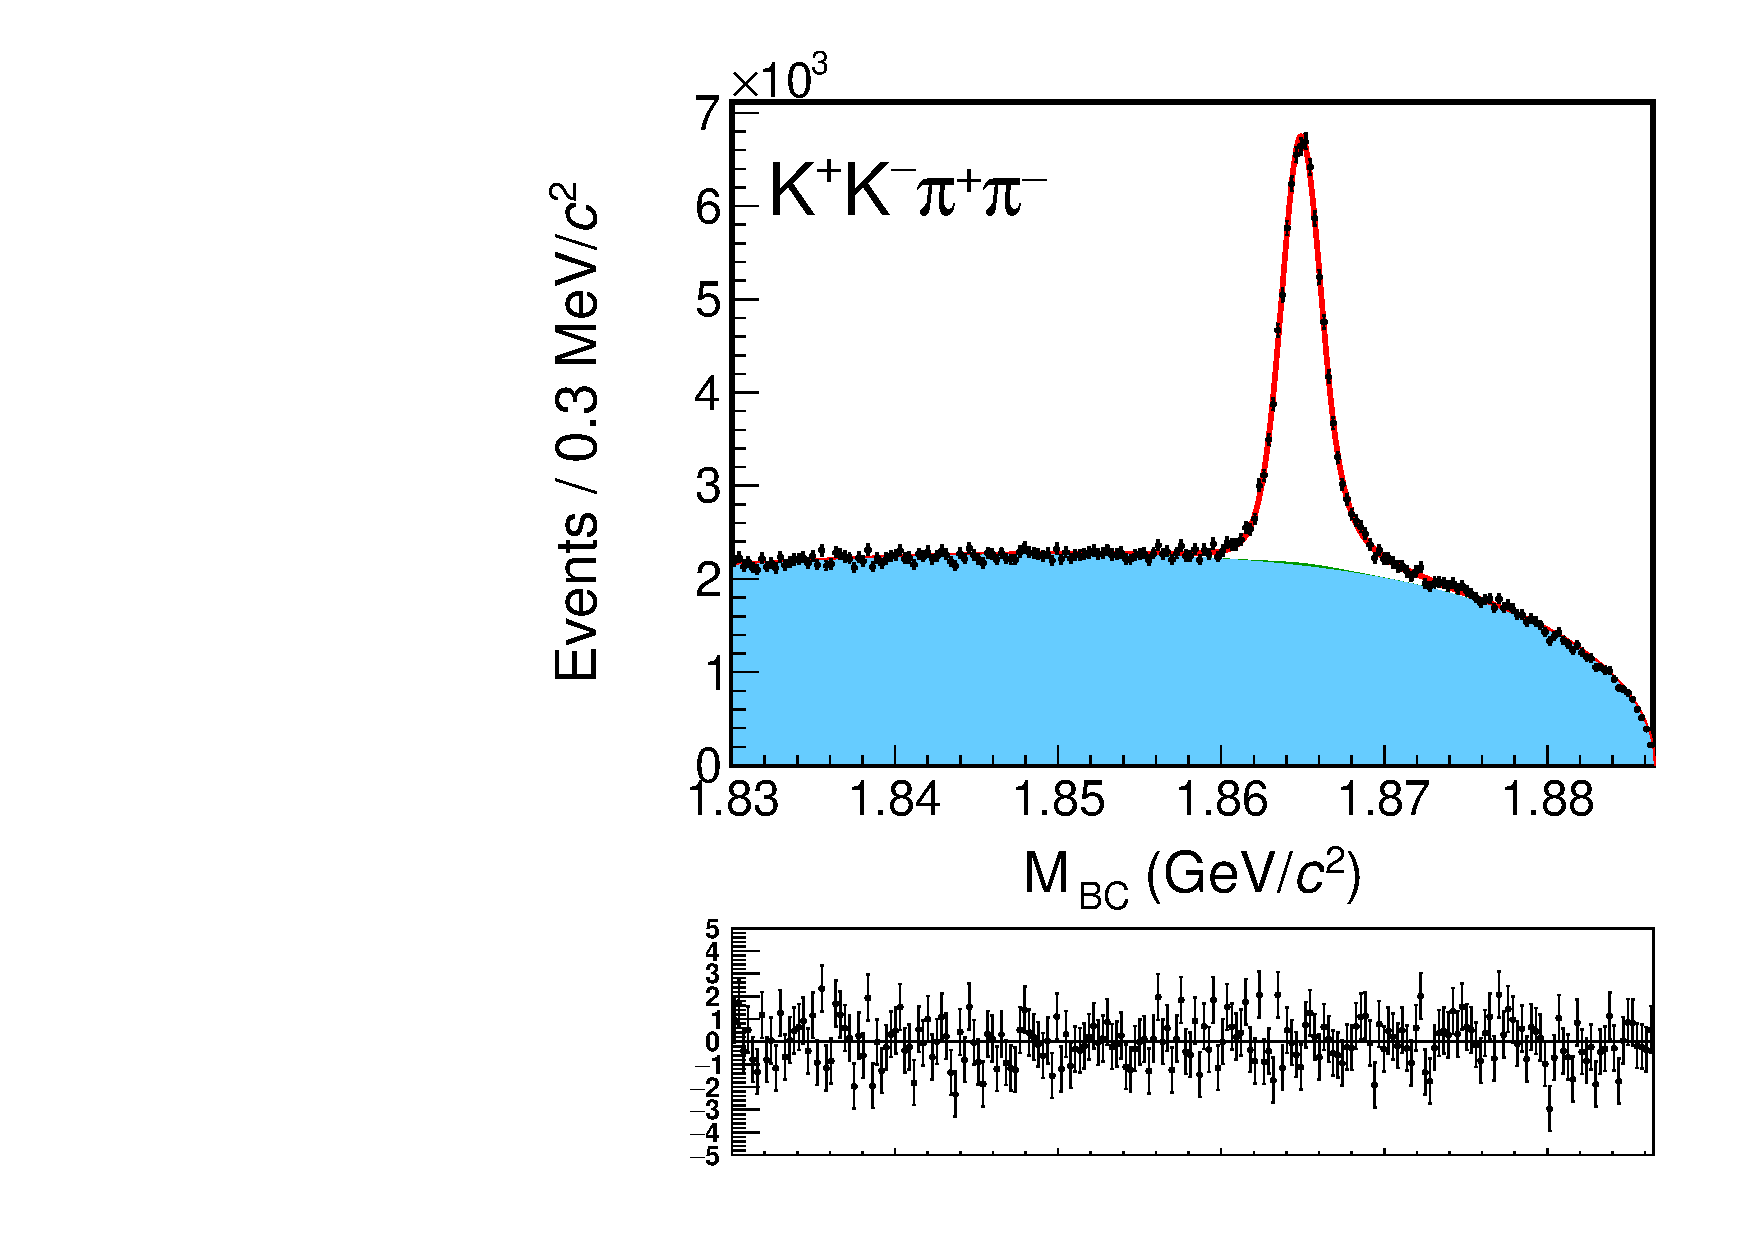
\includegraphics[width = 1.0\textwidth]{Plots/KKpipi_SingleTag_MBC_Plot_16invfb.pdf}
      \caption{$N = 59057 \pm 380$}
    \end{subfigure}
    \caption{Ratio of new and old ST $KK\pi\pi$ yield: $2.021 \pm 0.023$}
  \end{figure}
\end{frame}

\begin{frame}{Cross check of all ST yields}
  \begin{center}
    {\large Check that all other ST yields are consistent}
  \end{center}
  \vspace{0.1cm}
  \begin{itemize}
    \item{Combined ratio of ST yields: $2.0256 \pm 0.0013$}
    \item{Ratio of integrated luminosity: $2.93 + 4.995 + 8.157/2.93 + 4.995 = 2.029$}
  \end{itemize}
  \begin{figure}
    \centering
    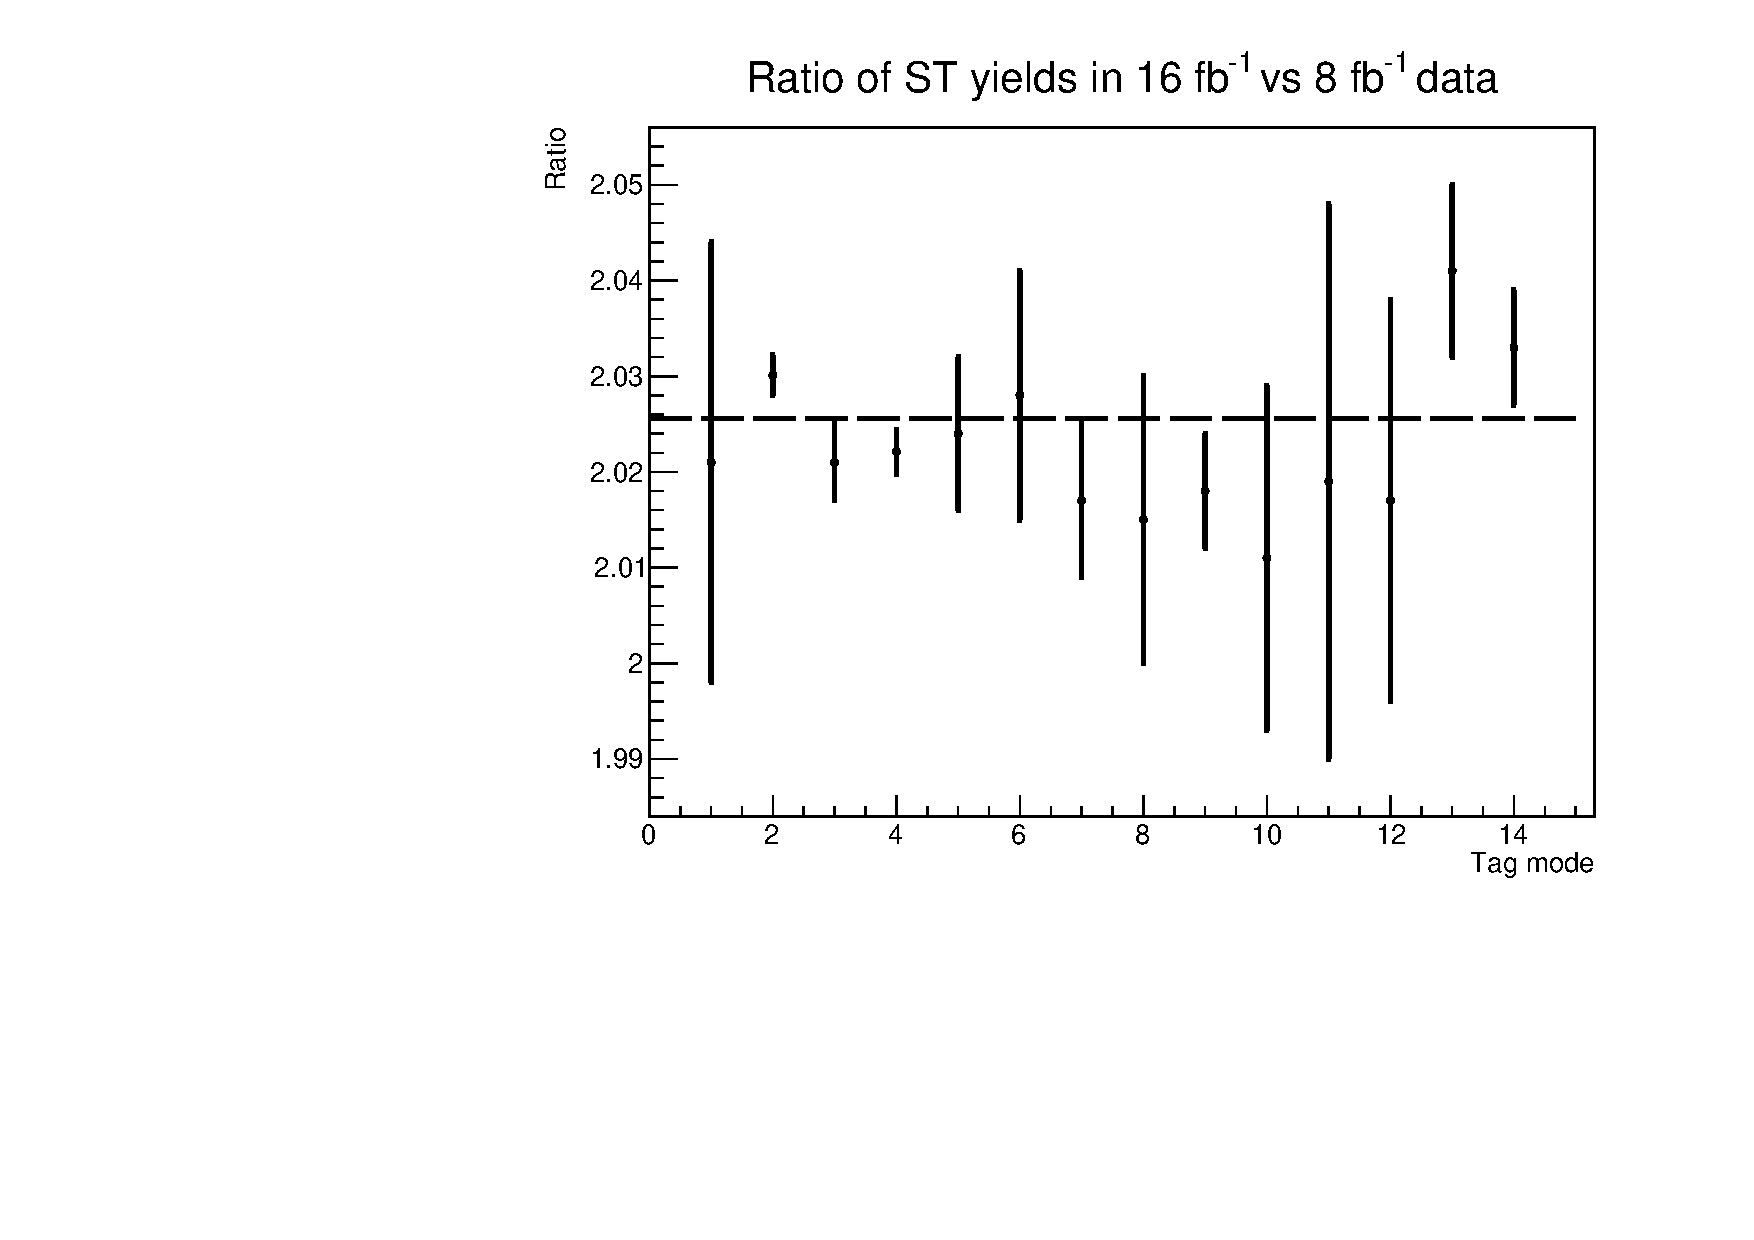
\includegraphics[width = 0.5\textwidth]{Plots/Ratio_ST_yields_16_8_invfb.pdf}
    \caption{Good agreement!}
  \end{figure}
\end{frame}

\begin{frame}{DT tag yields of $D^0\to K^+K^-\pi^+\pi^-$ with new data}
  \begin{center}
    {\large What about DT yields in phase-space bins?}
  \end{center}
  \vspace{0.1cm}
  \begin{figure}
    \centering
    \begin{subfigure}{0.45\textwidth}
      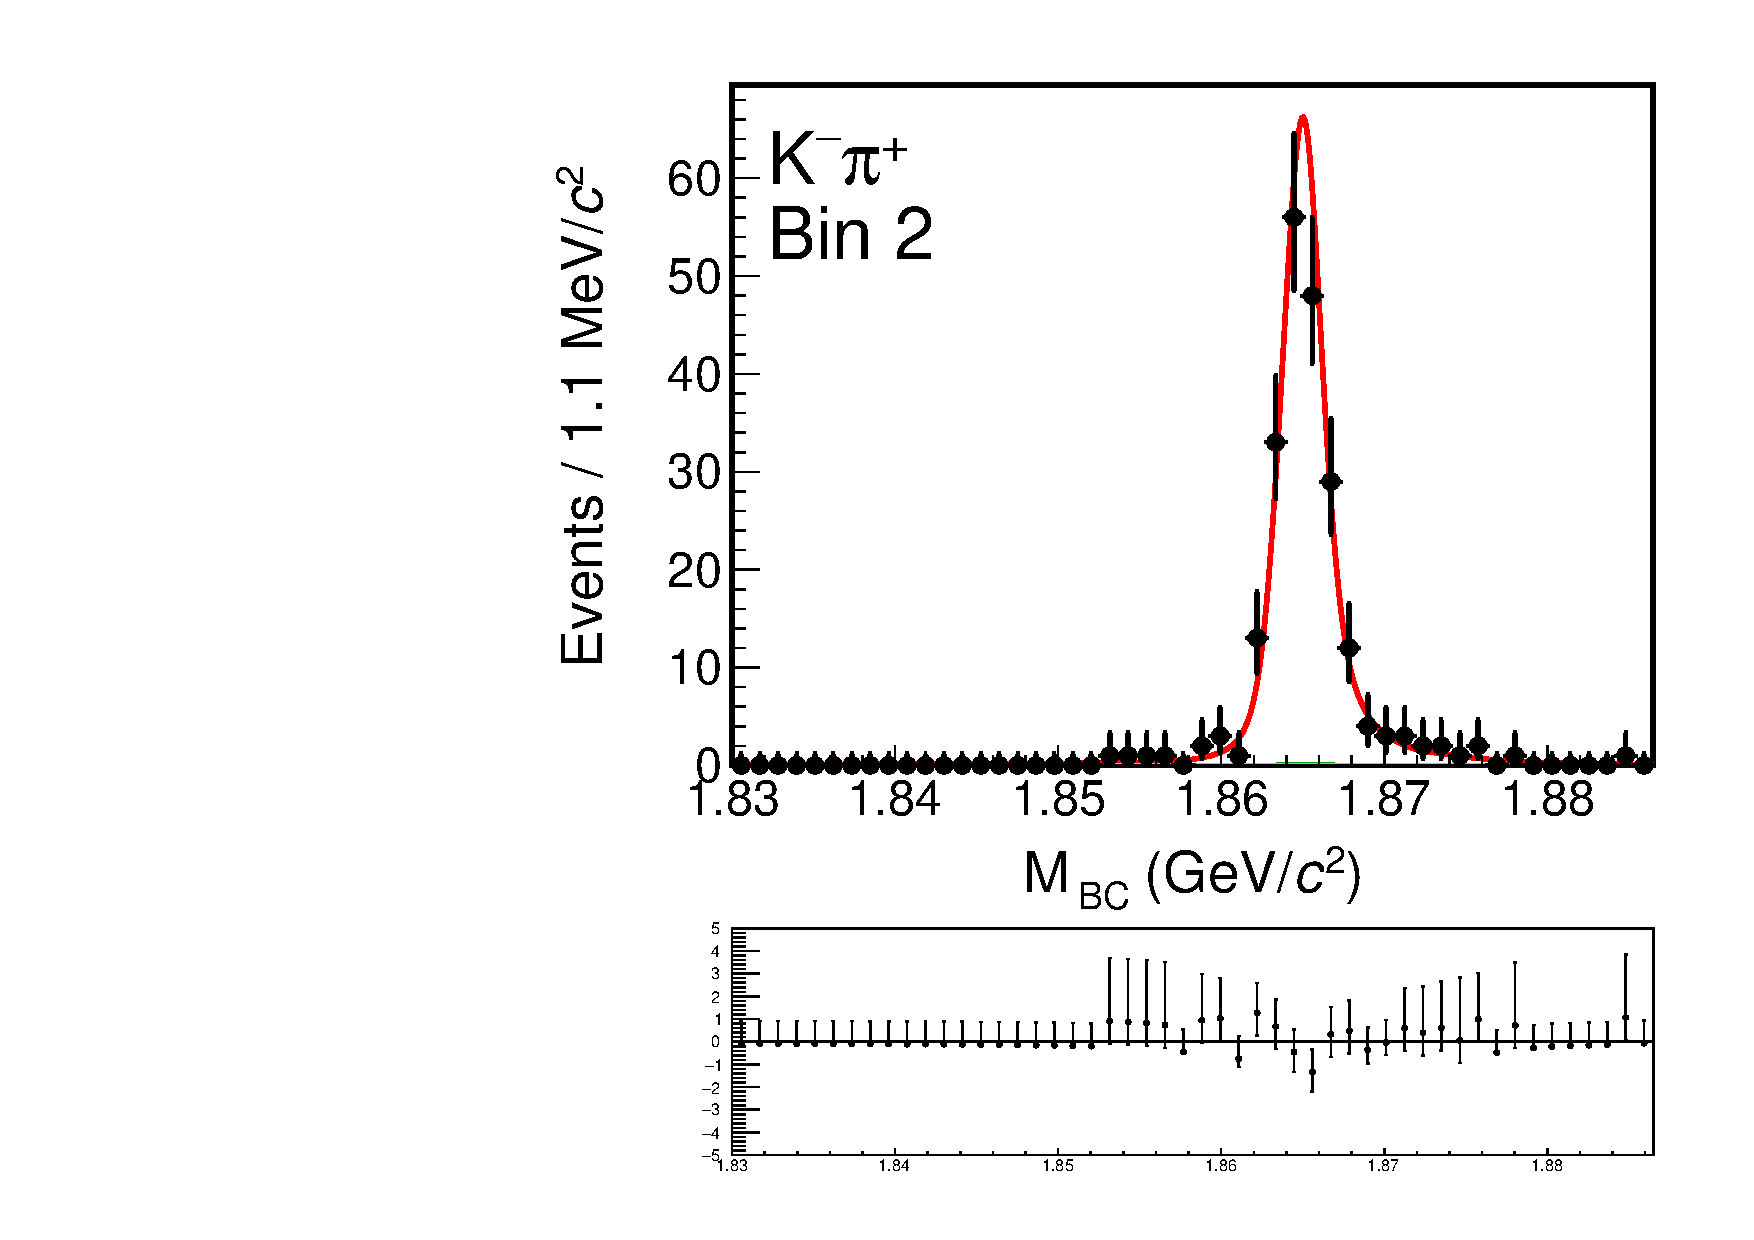
\includegraphics[width = 1.0\textwidth,trim={0 4.9cm 0 0},clip=true]{Plots/DoubleTagYield_DoubleTag_Flavour_KKpipi_vs_Kpi_SignalBinP2_TagBin0_8invfb.pdf}
      \caption{$N = 211.2^{+15.4}_{-14.8}$}
    \end{subfigure}%
    \hspace{1cm}
    \begin{subfigure}{0.45\textwidth}
      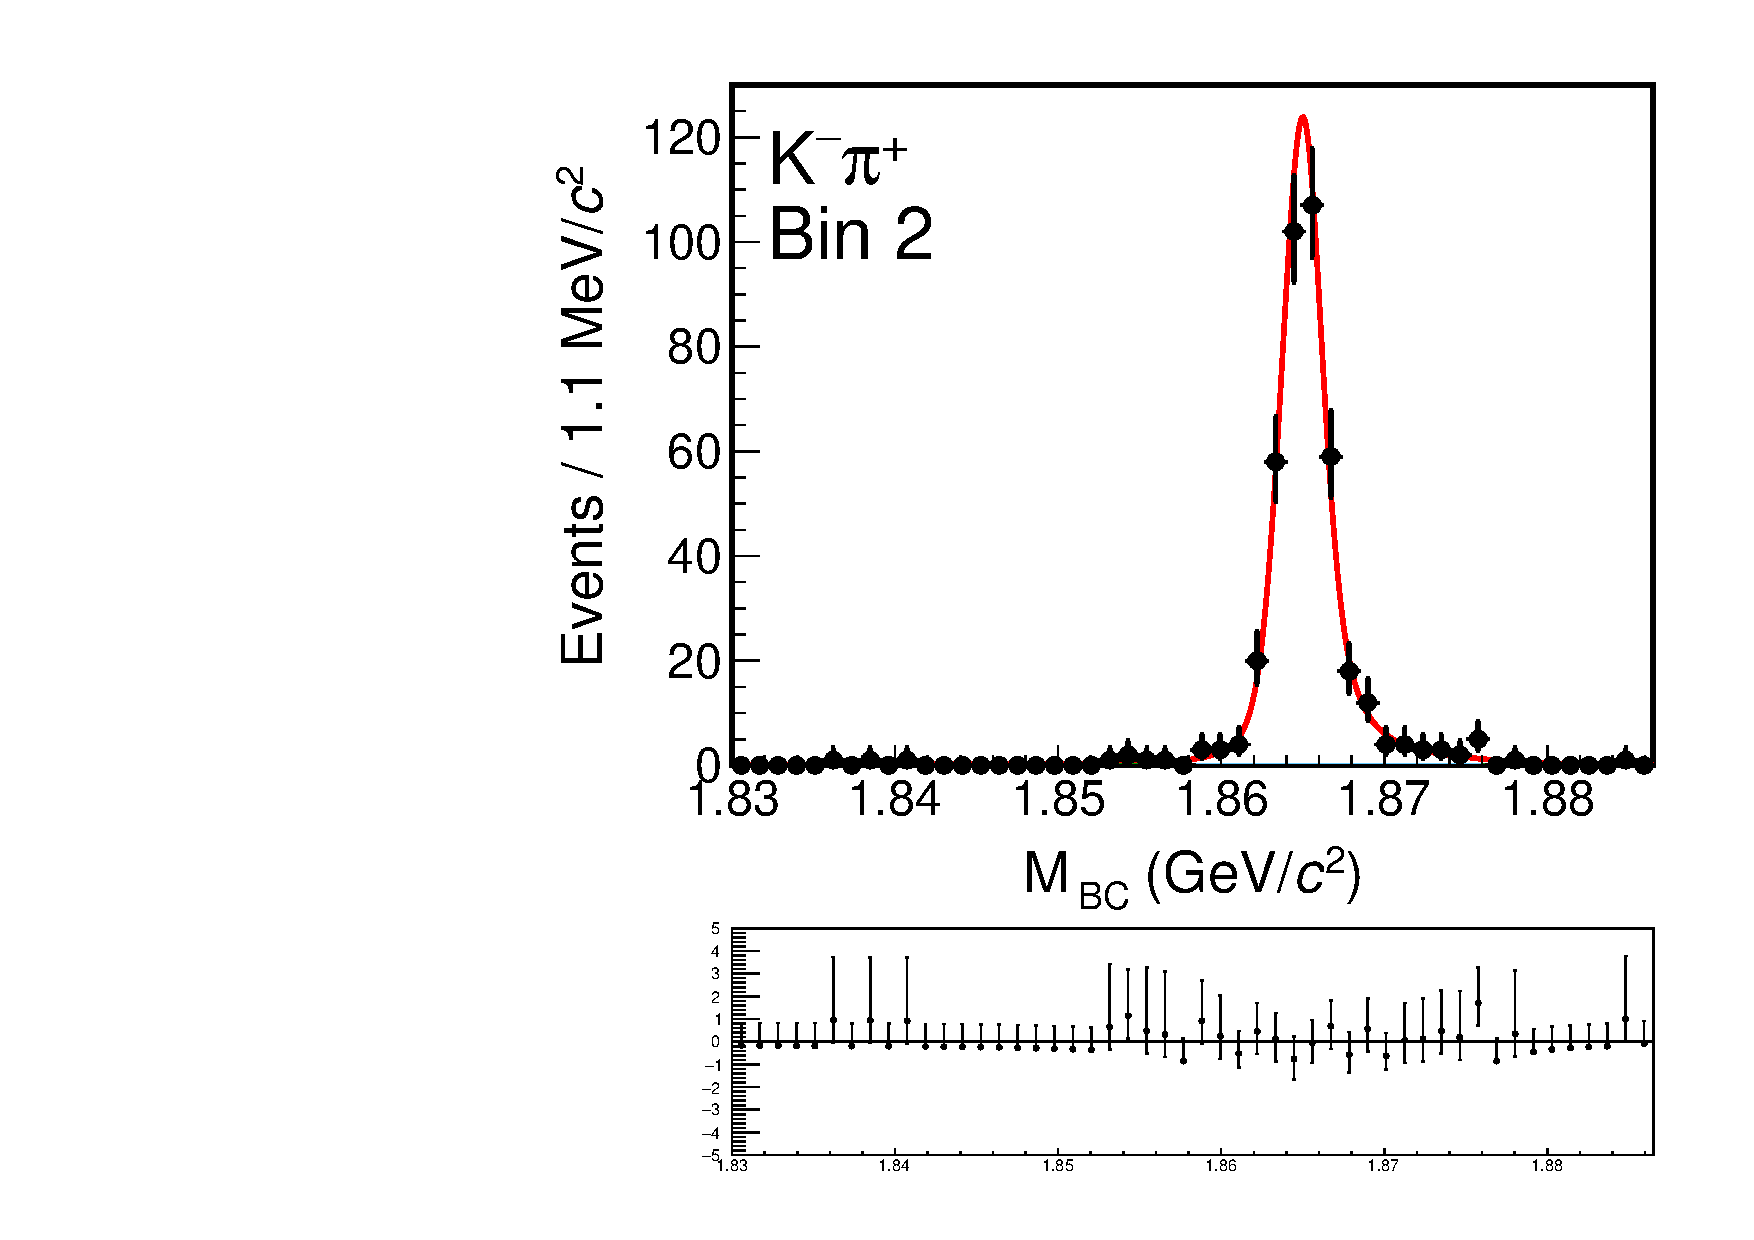
\includegraphics[width = 1.0\textwidth,trim={0 4.9cm 0 0},clip=true]{Plots/DoubleTagYield_DoubleTag_Flavour_KKpipi_vs_Kpi_SignalBinP2_TagBin0_16invfb.pdf}
      \caption{$N = 402.5^{+20.8}_{-20.2}$}
    \end{subfigure}
    \caption{Flavour tag $D\to K\pi$ with $\SI{8}{\per\femto\barn}$ ($\SI{16}{\per\femto\barn}$) on the left (right)}
  \end{figure}
\end{frame}

\begin{frame}{DT tag yields of $D^0\to K^+K^-\pi^+\pi^-$ with new data}
  \begin{center}
    {\large Check CP tags, which contain important strong-phase information}
  \end{center}
  \vspace{0.1cm}
  \begin{figure}
    \centering
    \begin{subfigure}{0.45\textwidth}
      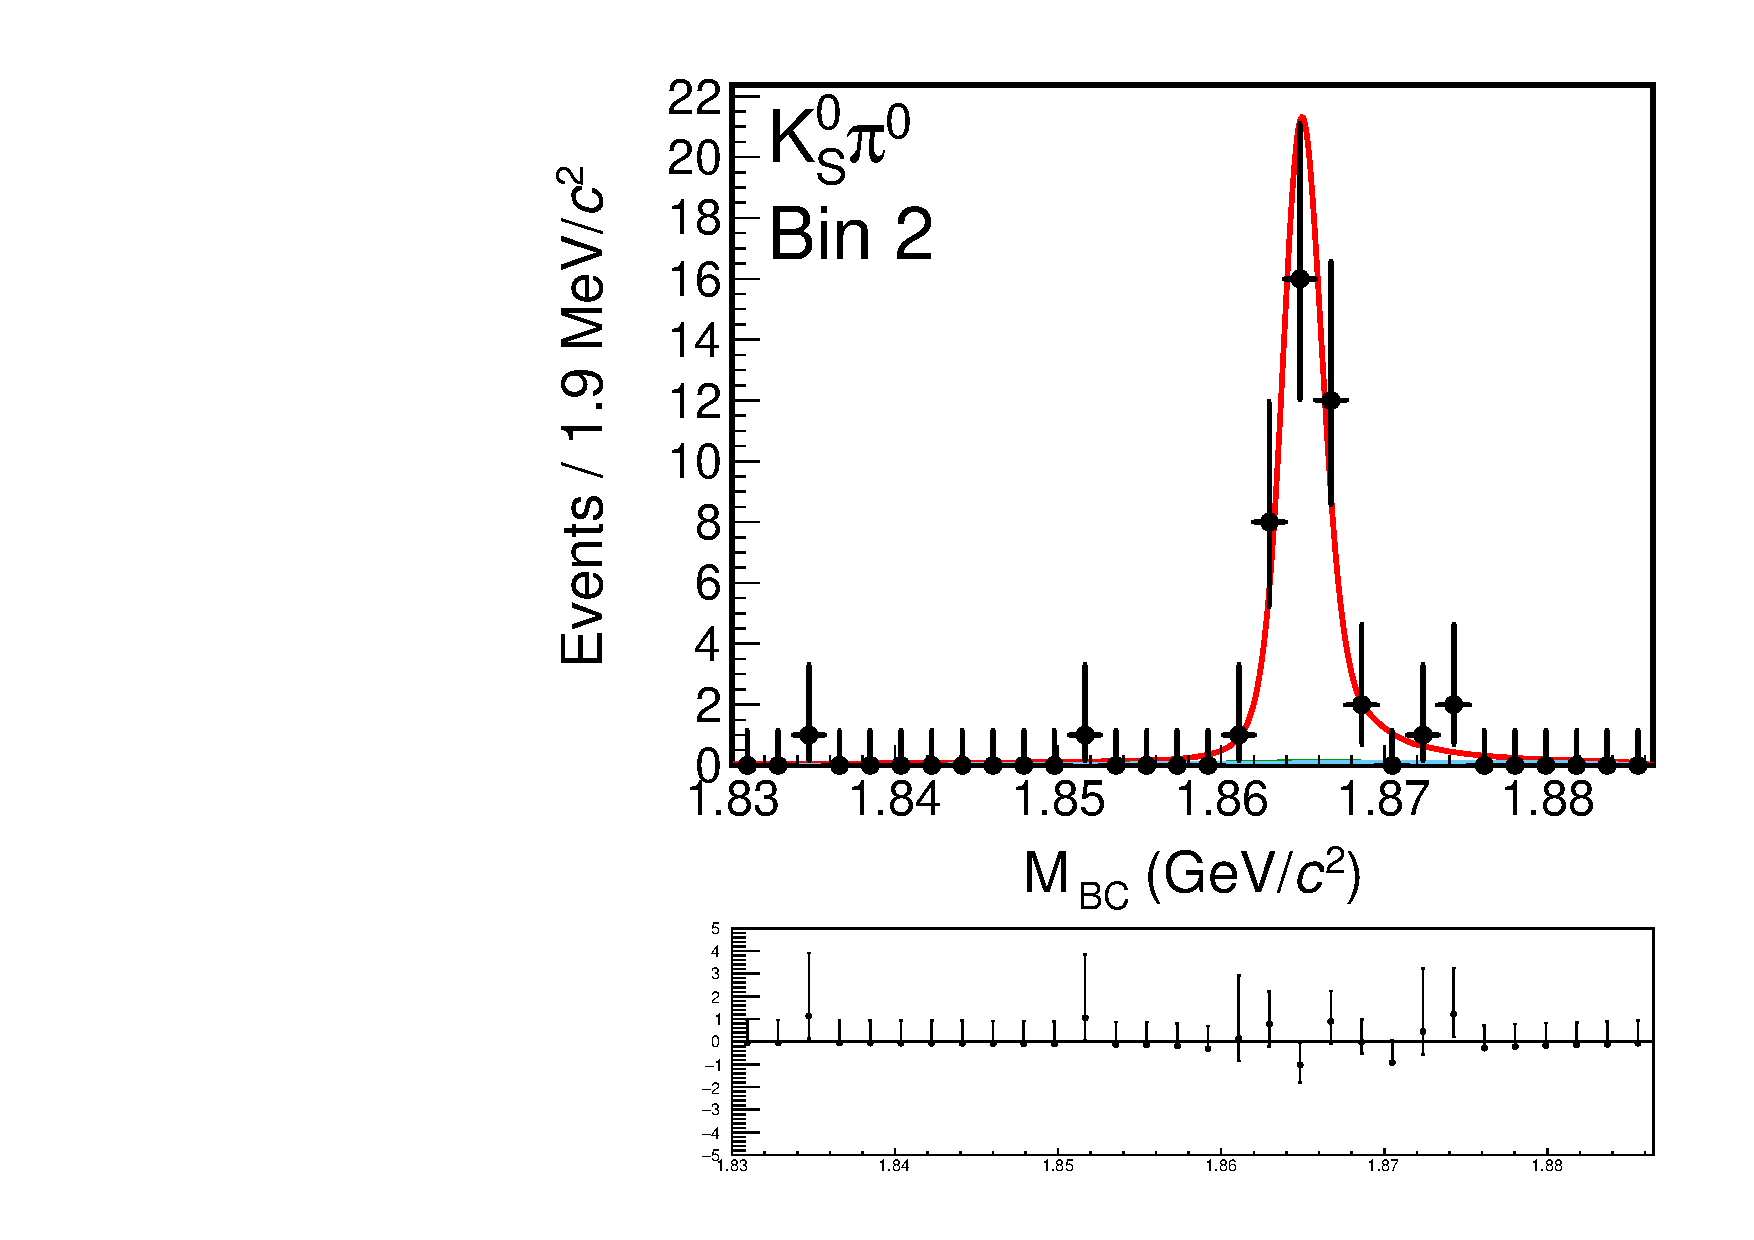
\includegraphics[width = 1.0\textwidth,trim={0 4.9cm 0 0},clip=true]{Plots/DoubleTagYield_DoubleTag_CP_KKpipi_vs_KSpi0_SignalBin2_8invfb.pdf}
      \caption{$N = 40.4^{+6.8}_{-6.3}$}
    \end{subfigure}%
    \hspace{1cm}
    \begin{subfigure}{0.45\textwidth}
      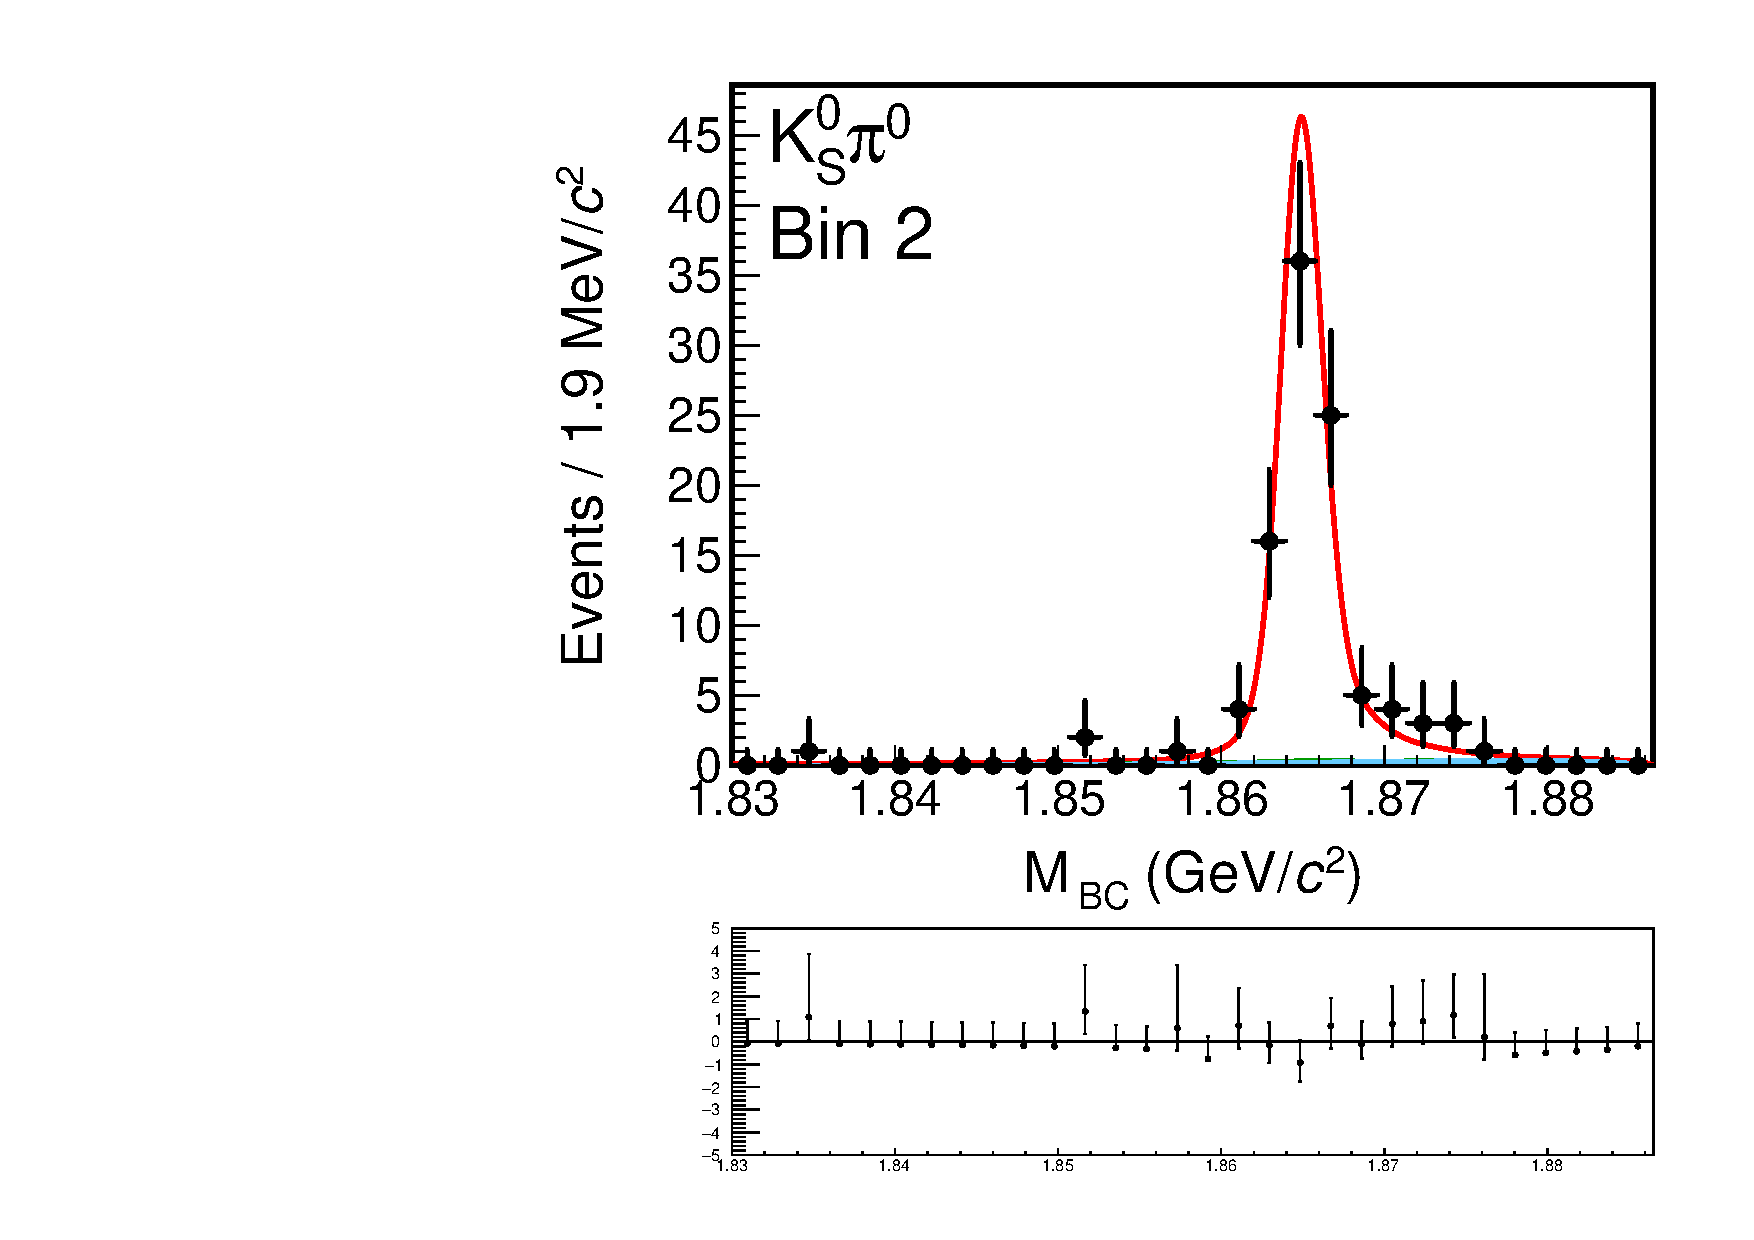
\includegraphics[width = 1.0\textwidth,trim={0 4.9cm 0 0},clip=true]{Plots/DoubleTagYield_DoubleTag_CP_KKpipi_vs_KSpi0_SignalBin2_16invfb.pdf}
      \caption{$N = 92.1^{+10.4}_{-9.9}$}
    \end{subfigure}
    \caption{CP tag $D\to K_S^0\pi^0$ with $\SI{8}{\per\femto\barn}$ ($\SI{16}{\per\femto\barn}$) on the left (right)}
  \end{figure}
\end{frame}

\begin{frame}{DT tag yields of $D^0\to K^+K^-\pi^+\pi^-$ with new data}
  \begin{center}
    {\large More importantly, what about multi-body tags?}
  \end{center}
  \vspace{0.1cm}
  \begin{figure}
    \centering
    \begin{subfigure}{0.45\textwidth}
      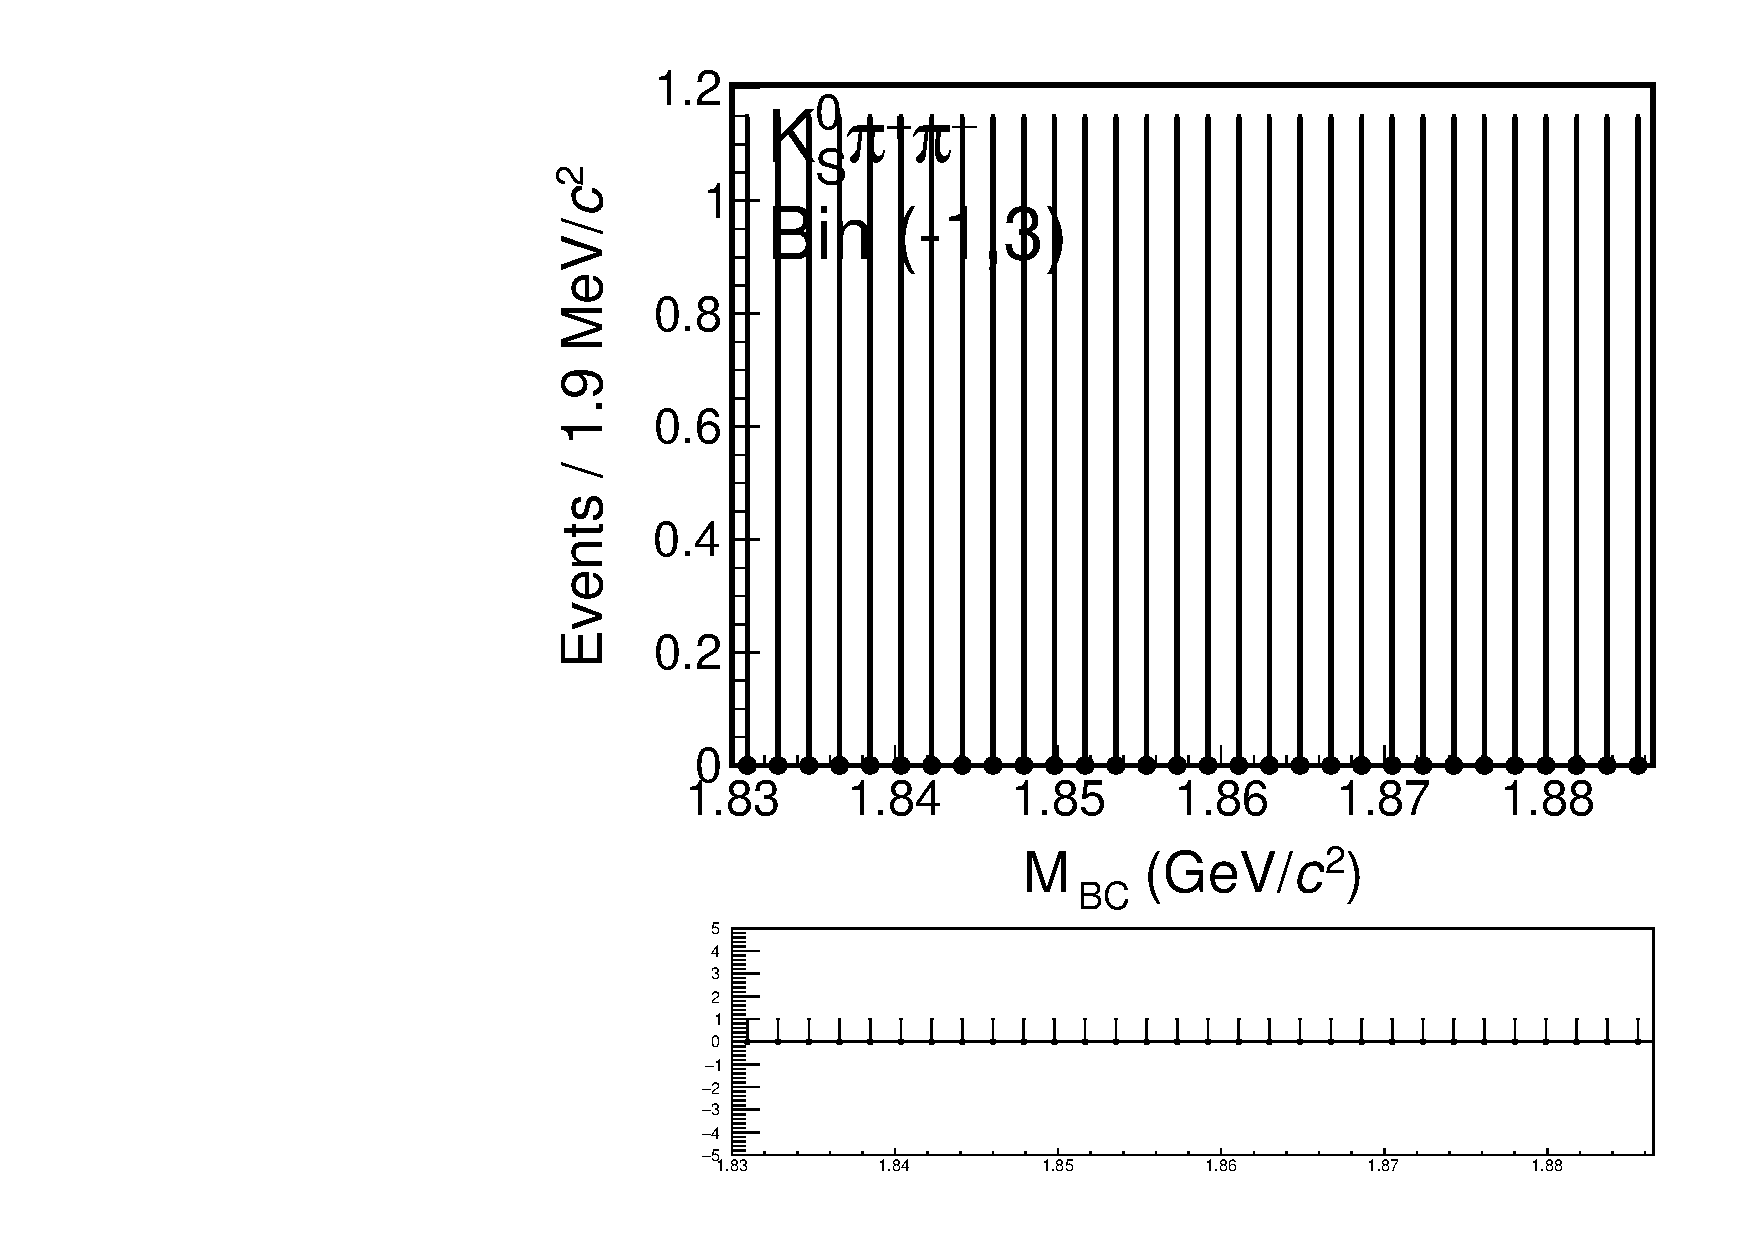
\includegraphics[width = 1.0\textwidth,trim={0 4.9cm 0 0},clip=true]{Plots/DoubleTagYield_DoubleTag_SCMB_KKpipi_vs_KSpipi_SignalBinM1_TagBin3_8invfb.pdf}
      \caption{$N = 0.0^{+0.5}_{-0.5}$}
    \end{subfigure}%
    \hspace{1cm}
    \begin{subfigure}{0.45\textwidth}
      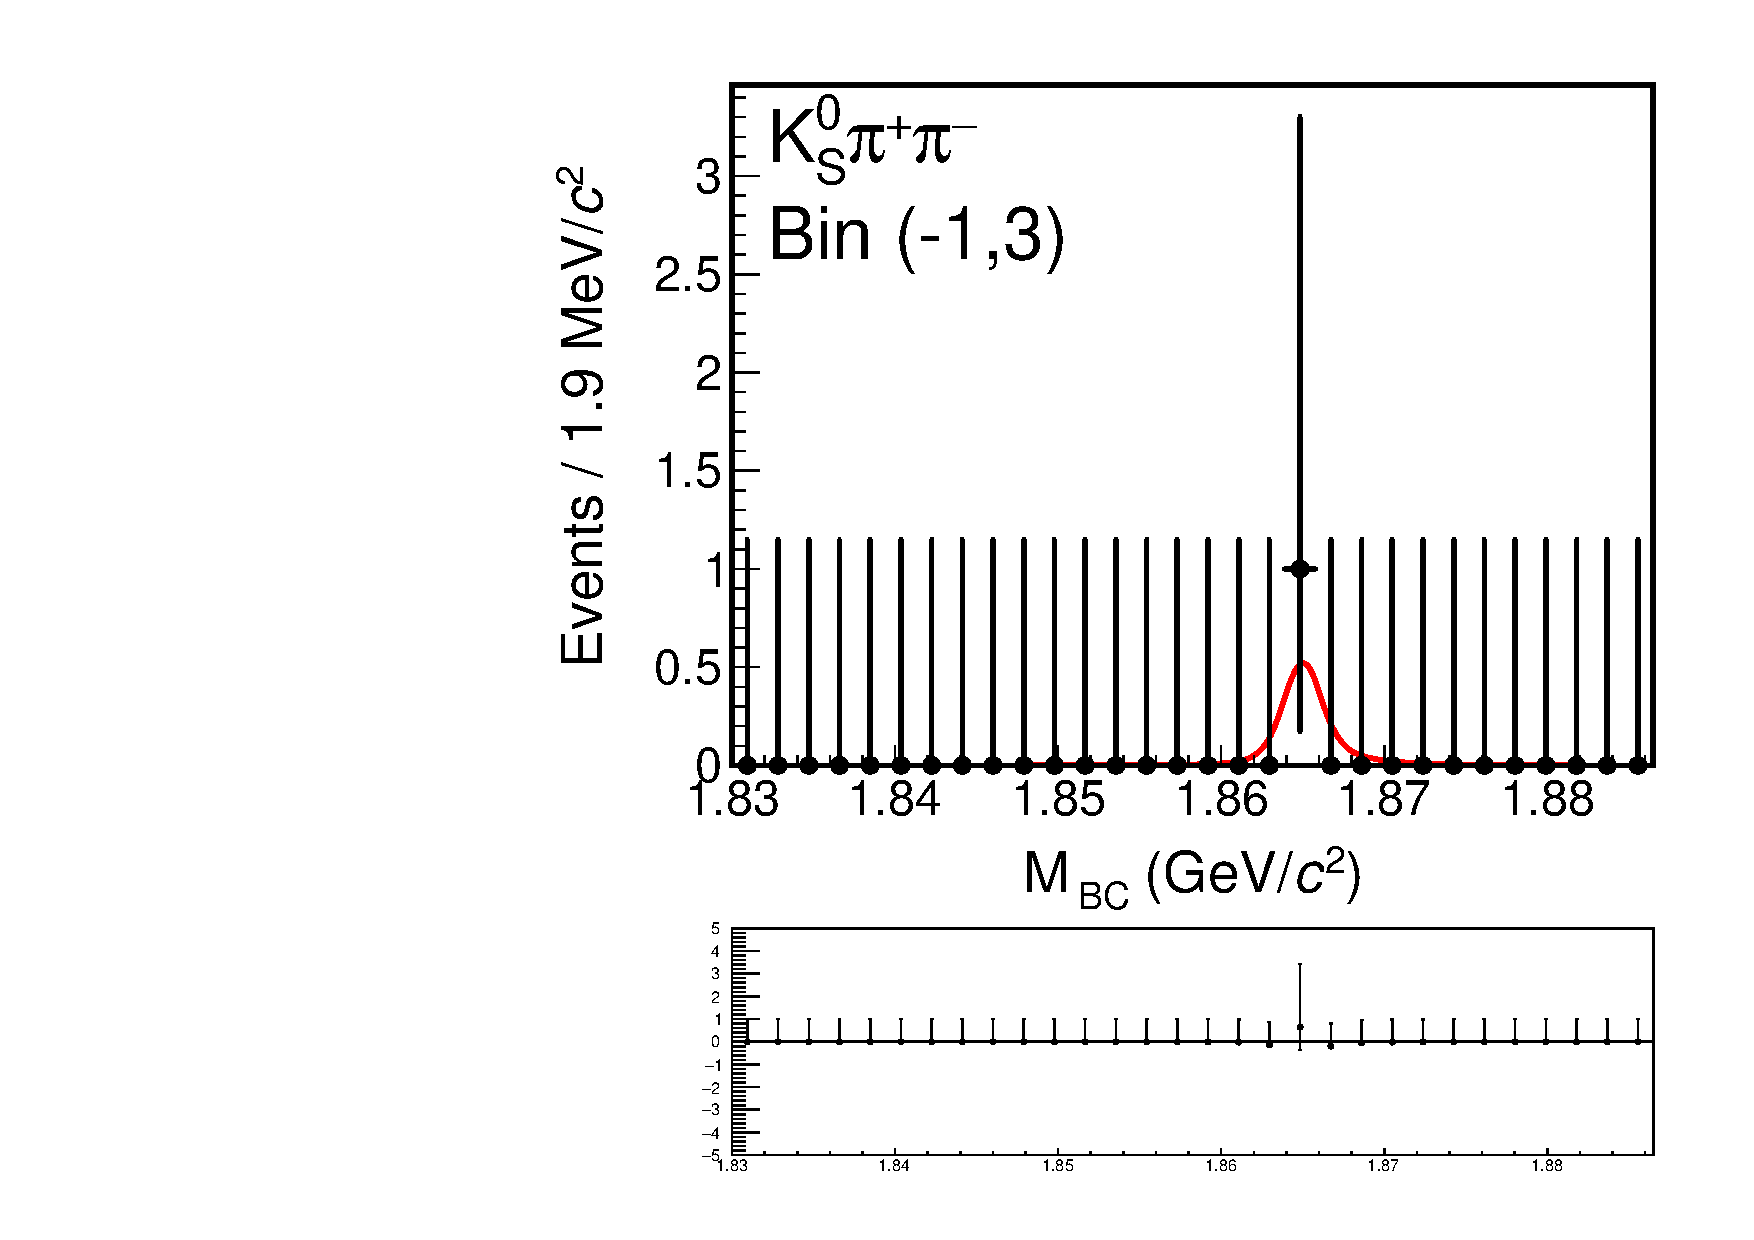
\includegraphics[width = 1.0\textwidth,trim={0 4.9cm 0 0},clip=true]{Plots/DoubleTagYield_DoubleTag_SCMB_KKpipi_vs_KSpipi_SignalBinM1_TagBin3_16invfb.pdf}
      \caption{$N = 1.0^{+1.3}_{-0.7}$}
    \end{subfigure}
    \caption{Multi-body tag $D\to K_S^0\pi^+\pi^-$ with $\SI{8}{\per\femto\barn}$ ($\SI{16}{\per\femto\barn}$) on the left (right)}
  \end{figure}
\end{frame}

\begin{frame}{DT tag yields of $D^0\to K^+K^-\pi^+\pi^-$ with new data}
  \begin{center}
    {\large More importantly, what about multi-body tags?}
  \end{center}
  \vspace{0.1cm}
  \begin{figure}
    \centering
    \begin{subfigure}{0.45\textwidth}
      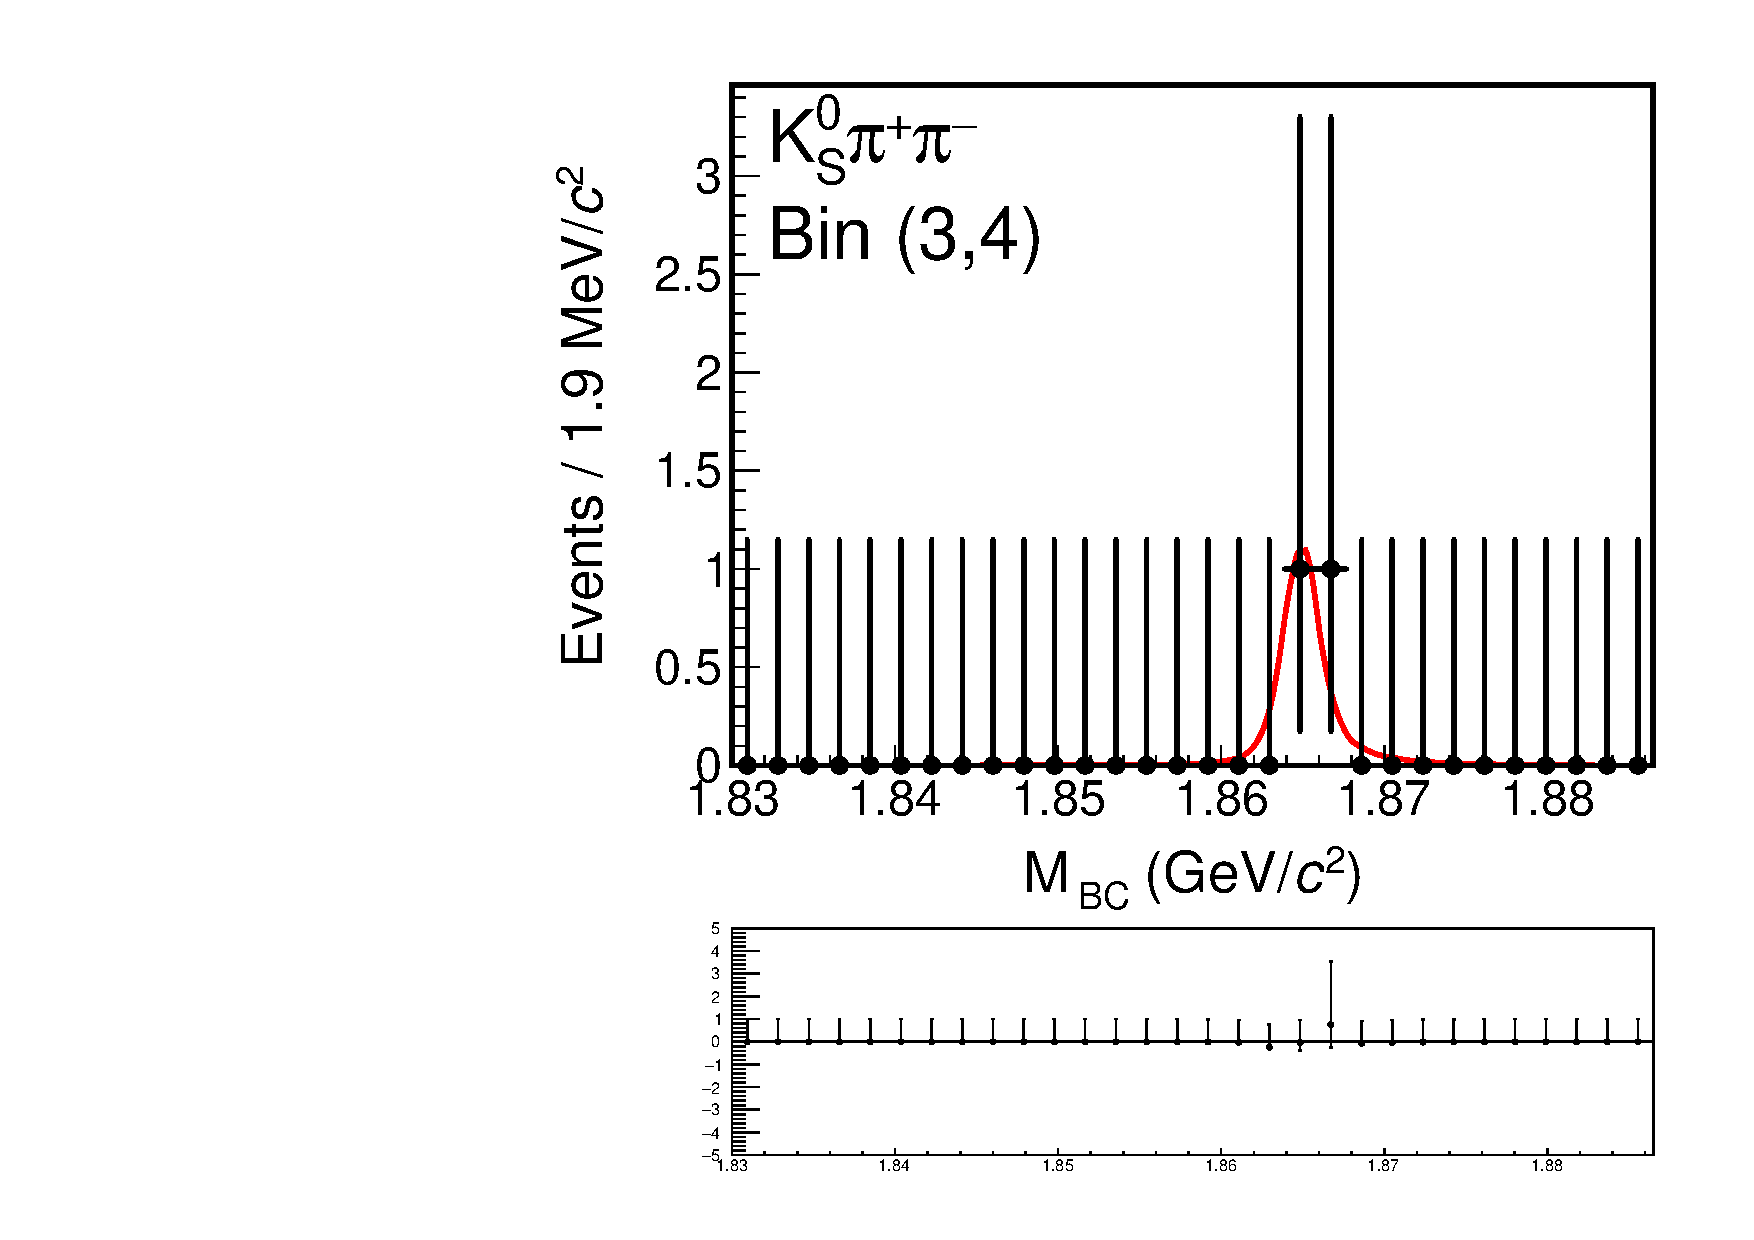
\includegraphics[width = 1.0\textwidth,trim={0 4.9cm 0 0},clip=true]{Plots/DoubleTagYield_DoubleTag_SCMB_KKpipi_vs_KSpipi_SignalBinP3_TagBin4_8invfb.pdf}
      \caption{$N = 2.0^{+1.8}_{-1.1}$}
    \end{subfigure}%
    \hspace{1cm}
    \begin{subfigure}{0.45\textwidth}
      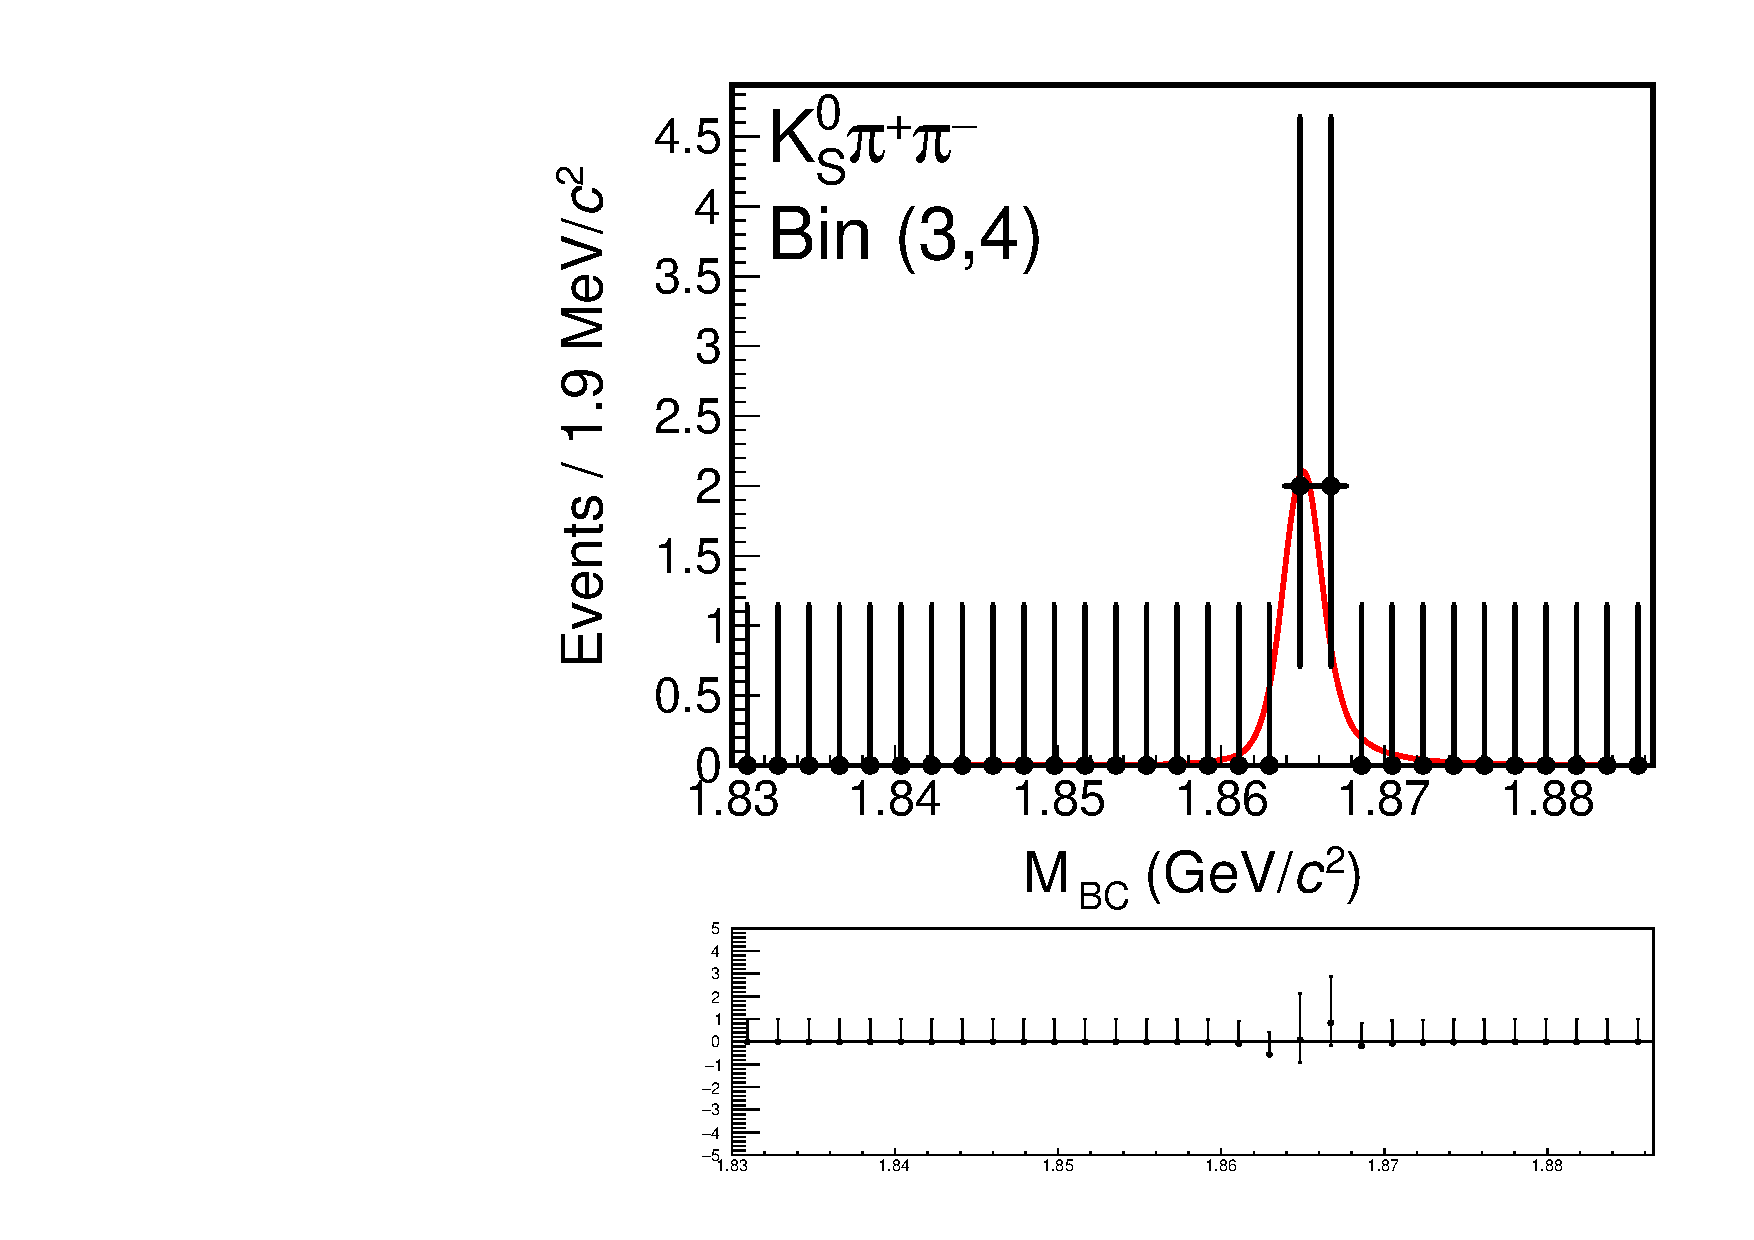
\includegraphics[width = 1.0\textwidth,trim={0 4.9cm 0 0},clip=true]{Plots/DoubleTagYield_DoubleTag_SCMB_KKpipi_vs_KSpipi_SignalBinP3_TagBin4_16invfb.pdf}
      \caption{$N = 4.0^{+2.3}_{-1.7}$}
    \end{subfigure}
    \caption{Multi-body tag $D\to K_S^0\pi^+\pi^-$ with $\SI{8}{\per\femto\barn}$ ($\SI{16}{\per\femto\barn}$) on the left (right)}
  \end{figure}
\end{frame}

\begin{frame}{Strong-phase fit with new data}
  \begin{center}
    \Large{What needs to be updated to fit $c_i$ and $s_i$?}
  \end{center}
  \vspace{0.1cm}
  \begin{enumerate}
    \setlength\itemsep{1.0em}
    \item{ST and DT yields (done!)}
    \item{Efficiency matrices (work in progress, probably negligible)}
    \begin{itemize}
      \item{Don't bother with new MC, just reweight 2022 MC with a factor $13/5$}
    \end{itemize}
    \item{Toy studies (work in progress)}
    \item{Tracking and PID efficiency systematics}
    \begin{itemize}
      \item{Can probably get away with reusing same numbers}
    \end{itemize}
  \end{enumerate}
\end{frame}

\begin{frame}{Strong-phase fit with new data}
  \begin{center}
    {\large Run fit of $c_i$ and $s_i$ with new ST and DT yields}
  \end{center}
  \vspace{-0.5cm}
  \begin{figure}
    \centering
    \begin{subfigure}{0.45\textwidth}
      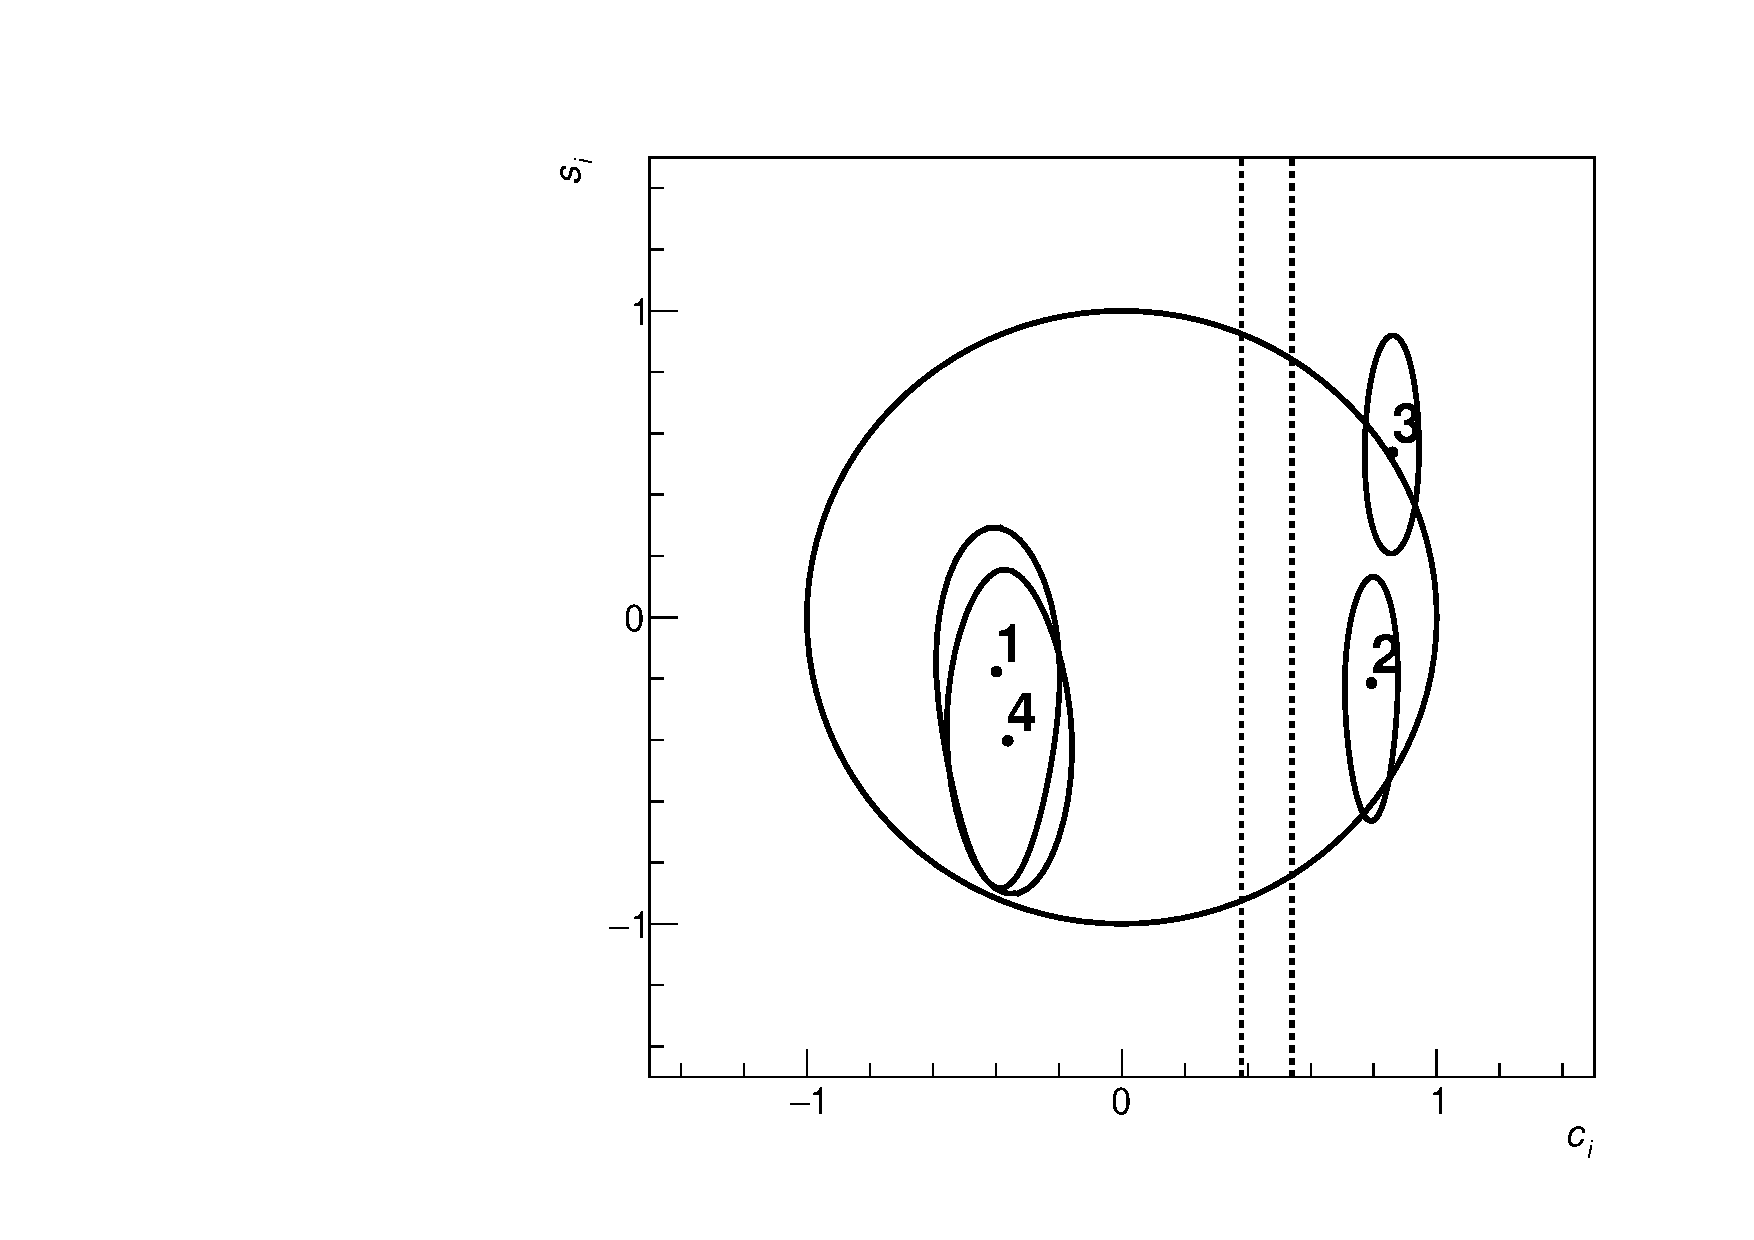
\includegraphics[width = 1.0\textwidth]{Plots/Contours_cisi_8invfb.pdf}
      \caption{$\SI{8}{\per\femto\barn}$}
    \end{subfigure}%
    \hspace{1cm}
    \begin{subfigure}{0.45\textwidth}
      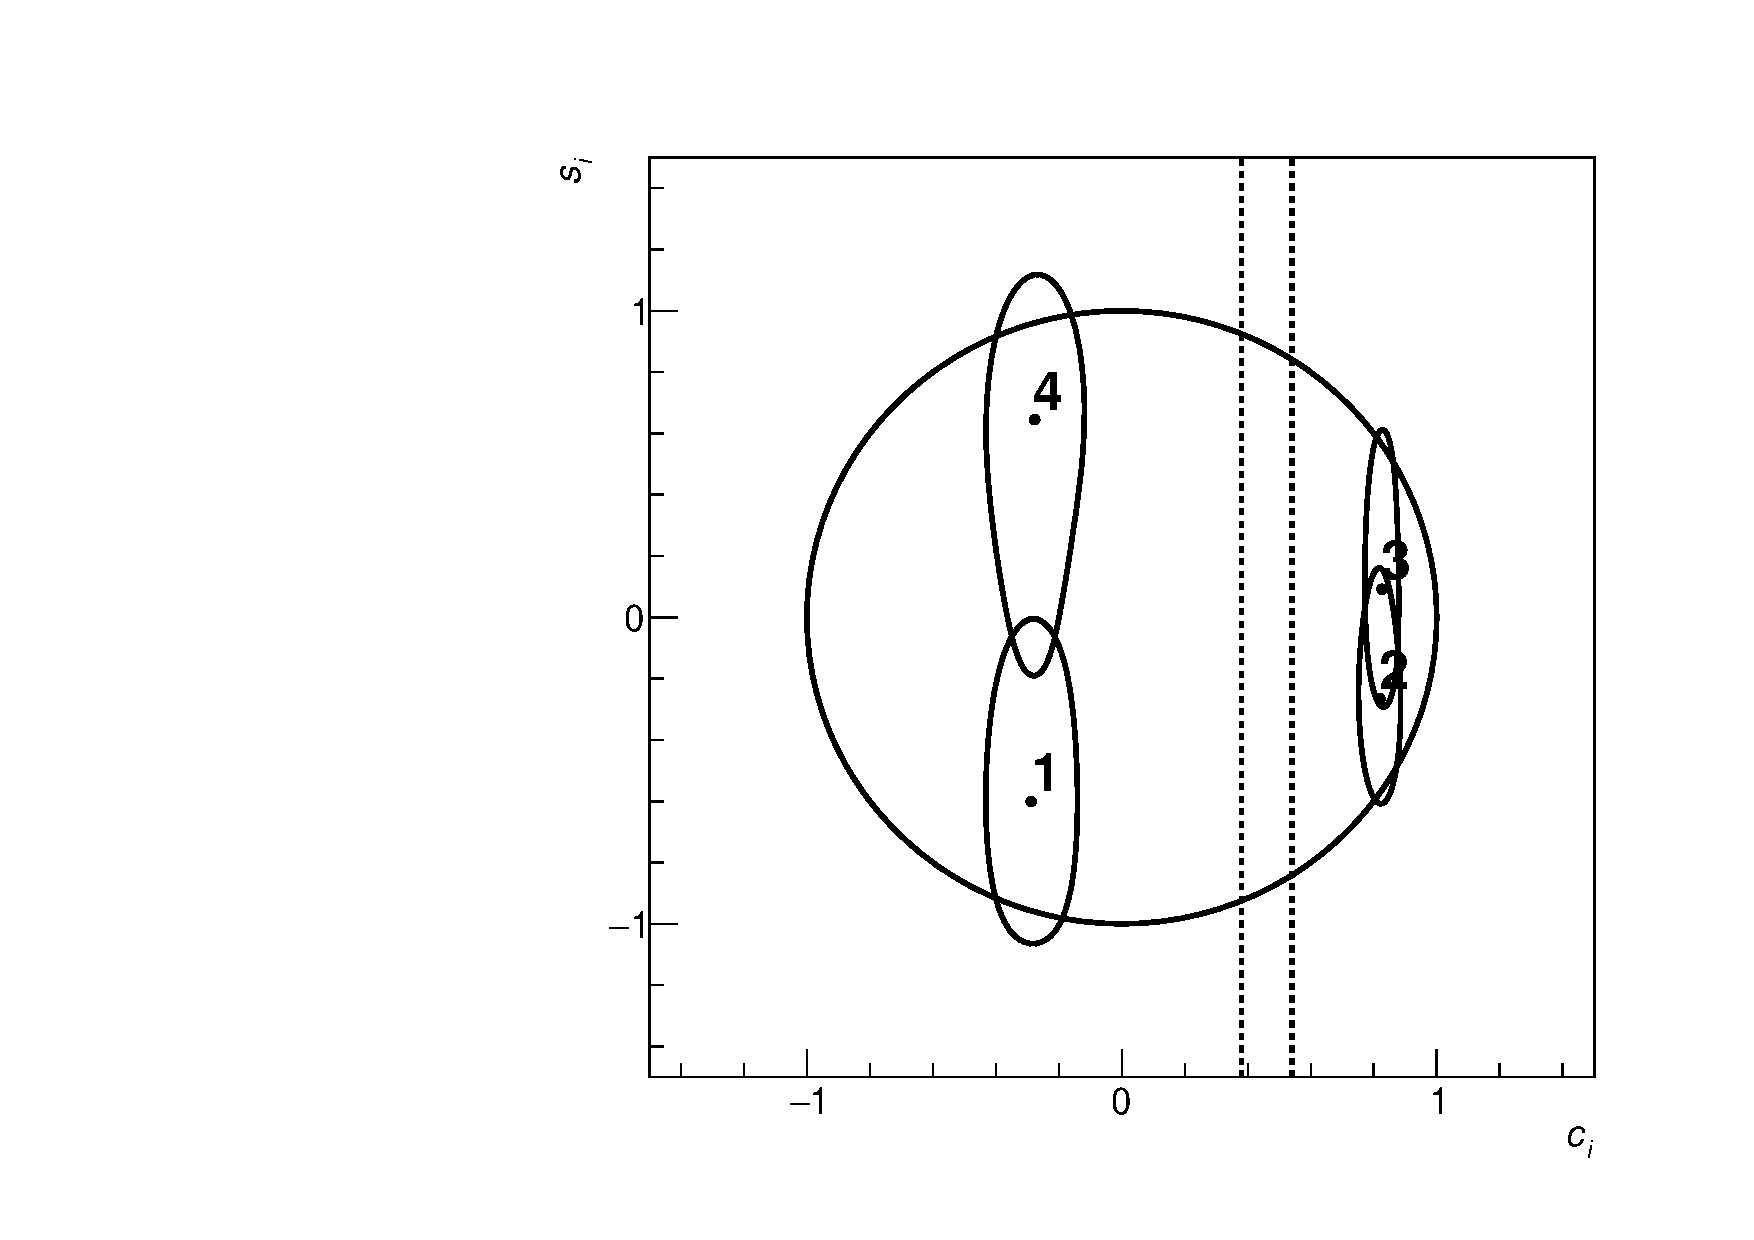
\includegraphics[width = 1.0\textwidth]{Plots/Contours_cisi_16invfb.pdf}
      \caption{$\SI{16}{\per\femto\barn}$}
    \end{subfigure}
    \caption{Warning: $s_i$ uncertainties may be very non-Gaussian}
  \end{figure}
\end{frame}

\begin{frame}{Strong-phase fit with new data}
  \begin{center}
    {\large New $c_i$ and $s_i$ results are perfectly consistent with model!}
  \end{center}
  \vspace{-0.5cm}
  \begin{figure}
    \centering
    \begin{subfigure}{0.45\textwidth}
      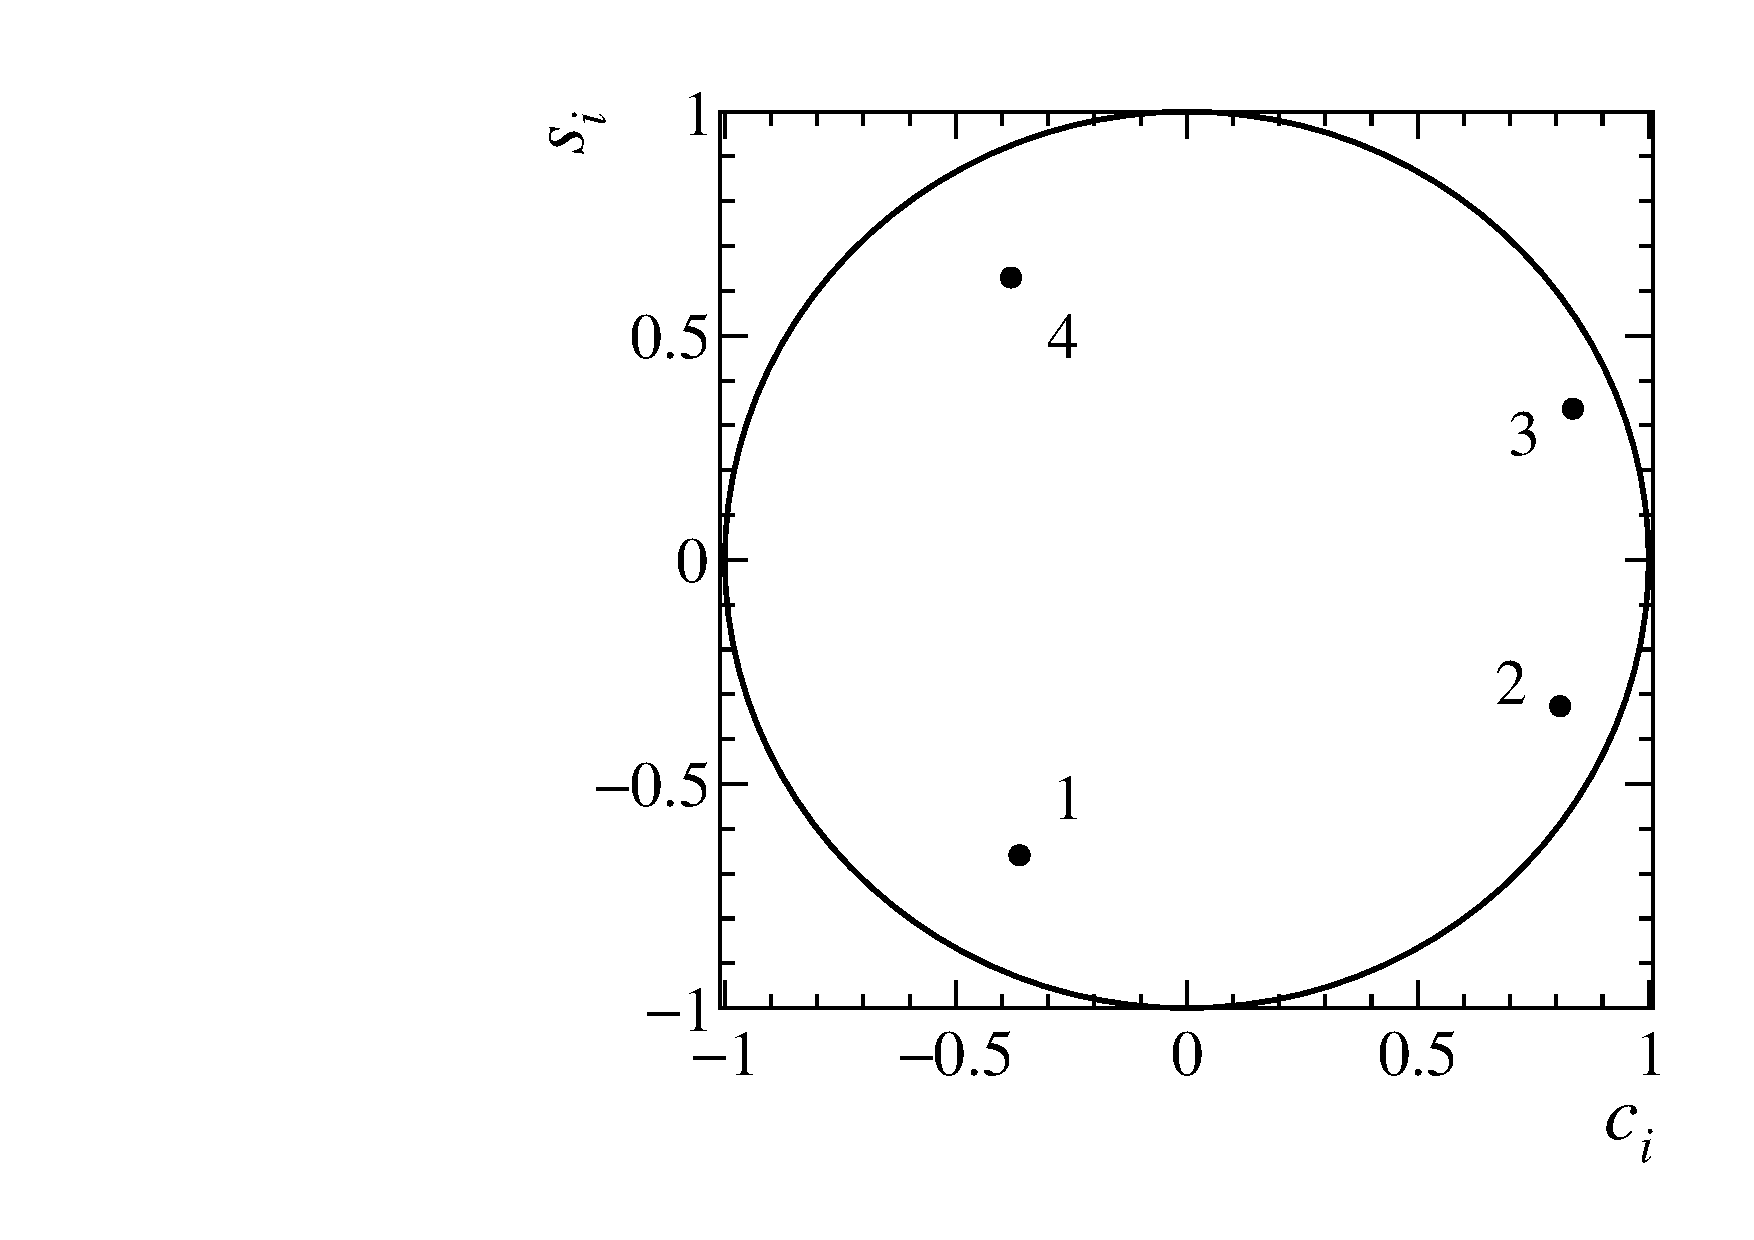
\includegraphics[width = 0.97\textwidth]{Plots/StrongPhaseParametersPlot_cisi_4Bins.pdf}
      \caption{Model predictions}
    \end{subfigure}%
    \hspace{1cm}
    \begin{subfigure}{0.45\textwidth}
      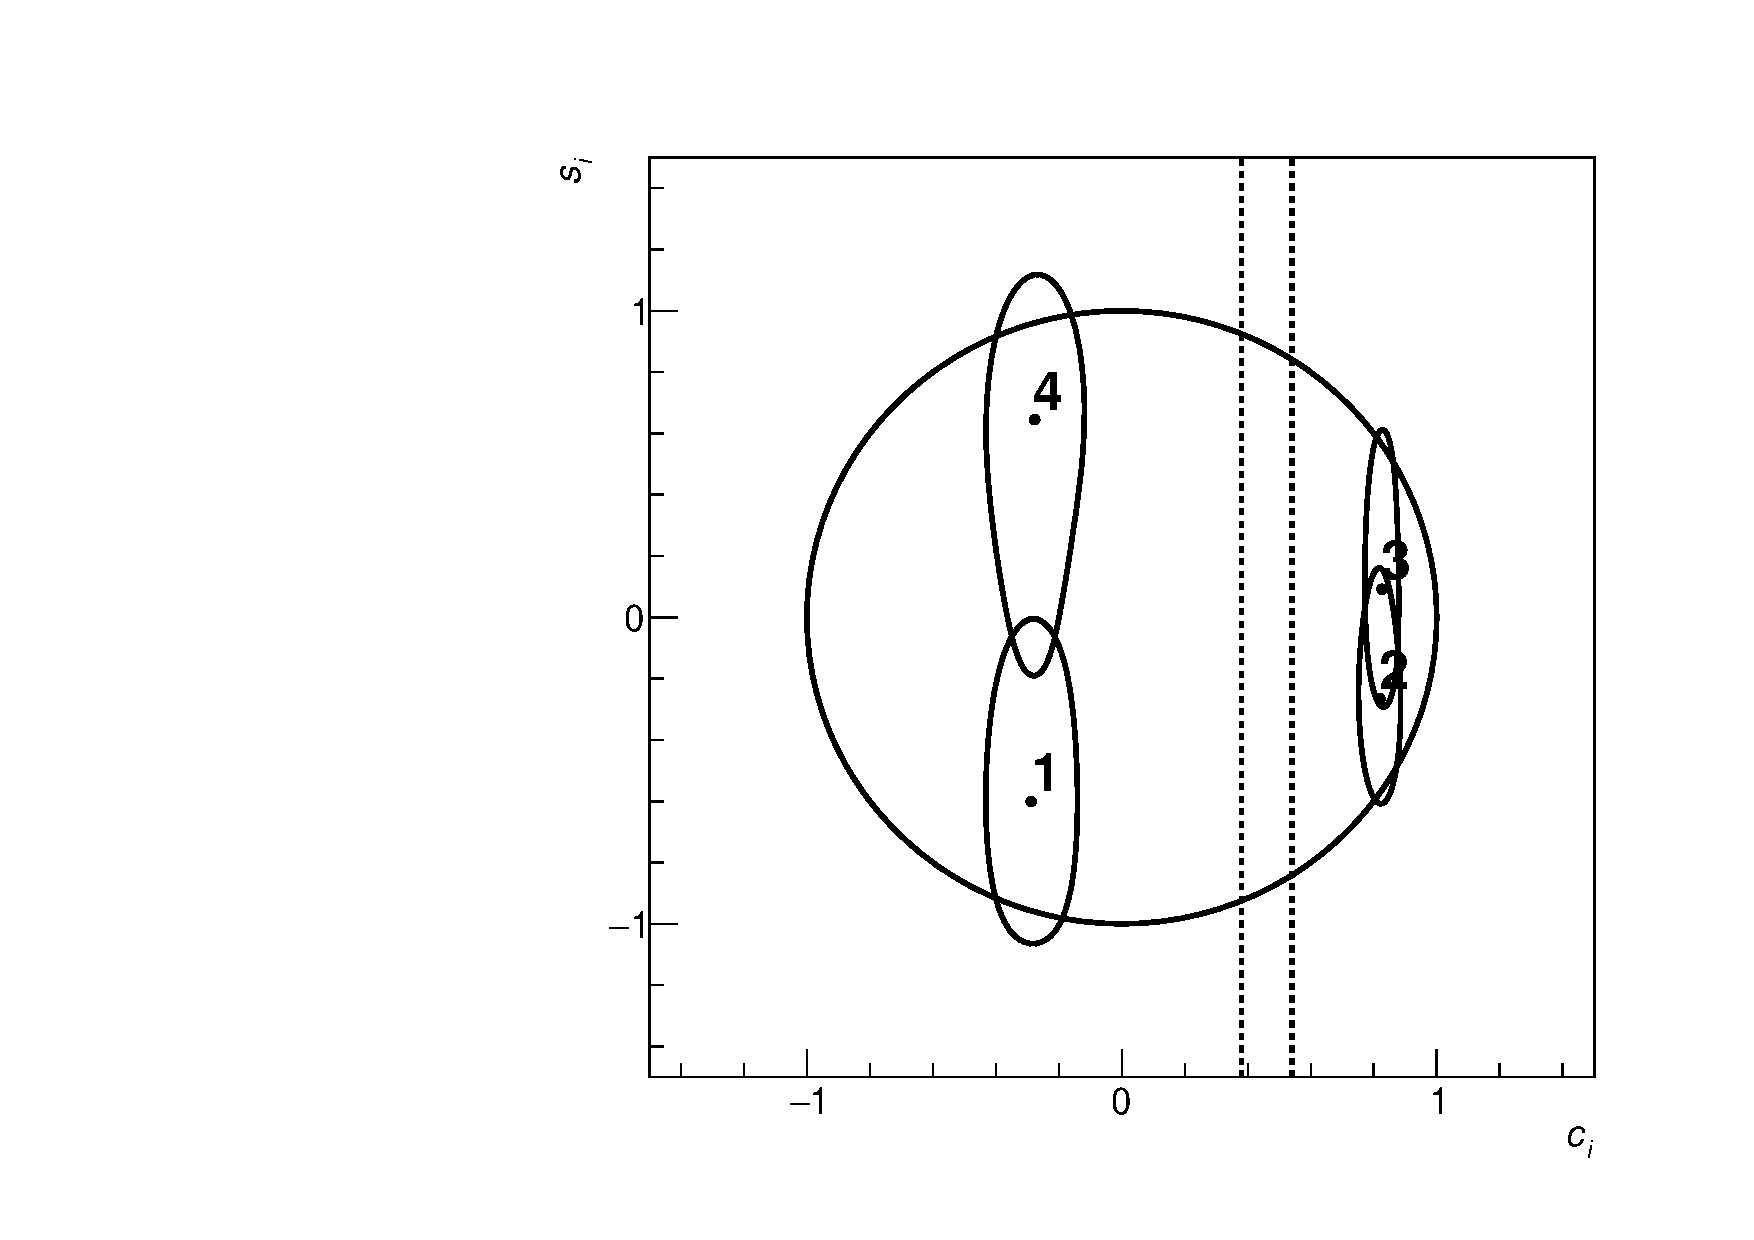
\includegraphics[width = 1.0\textwidth]{Plots/Contours_cisi_16invfb.pdf}
      \caption{$\SI{16}{\per\femto\barn}$}
    \end{subfigure}
    \caption{Warning: $s_i$ uncertainties may be very non-Gaussian}
  \end{figure}
\end{frame}

\begin{frame}{Strong-phase fit with new data}
  \begin{center}
    {\large What about $\delta_D^{K\pi}$?}
  \end{center}
  \vspace{-0.5cm}
  \begin{figure}
    \centering
    \begin{subfigure}{0.45\textwidth}
      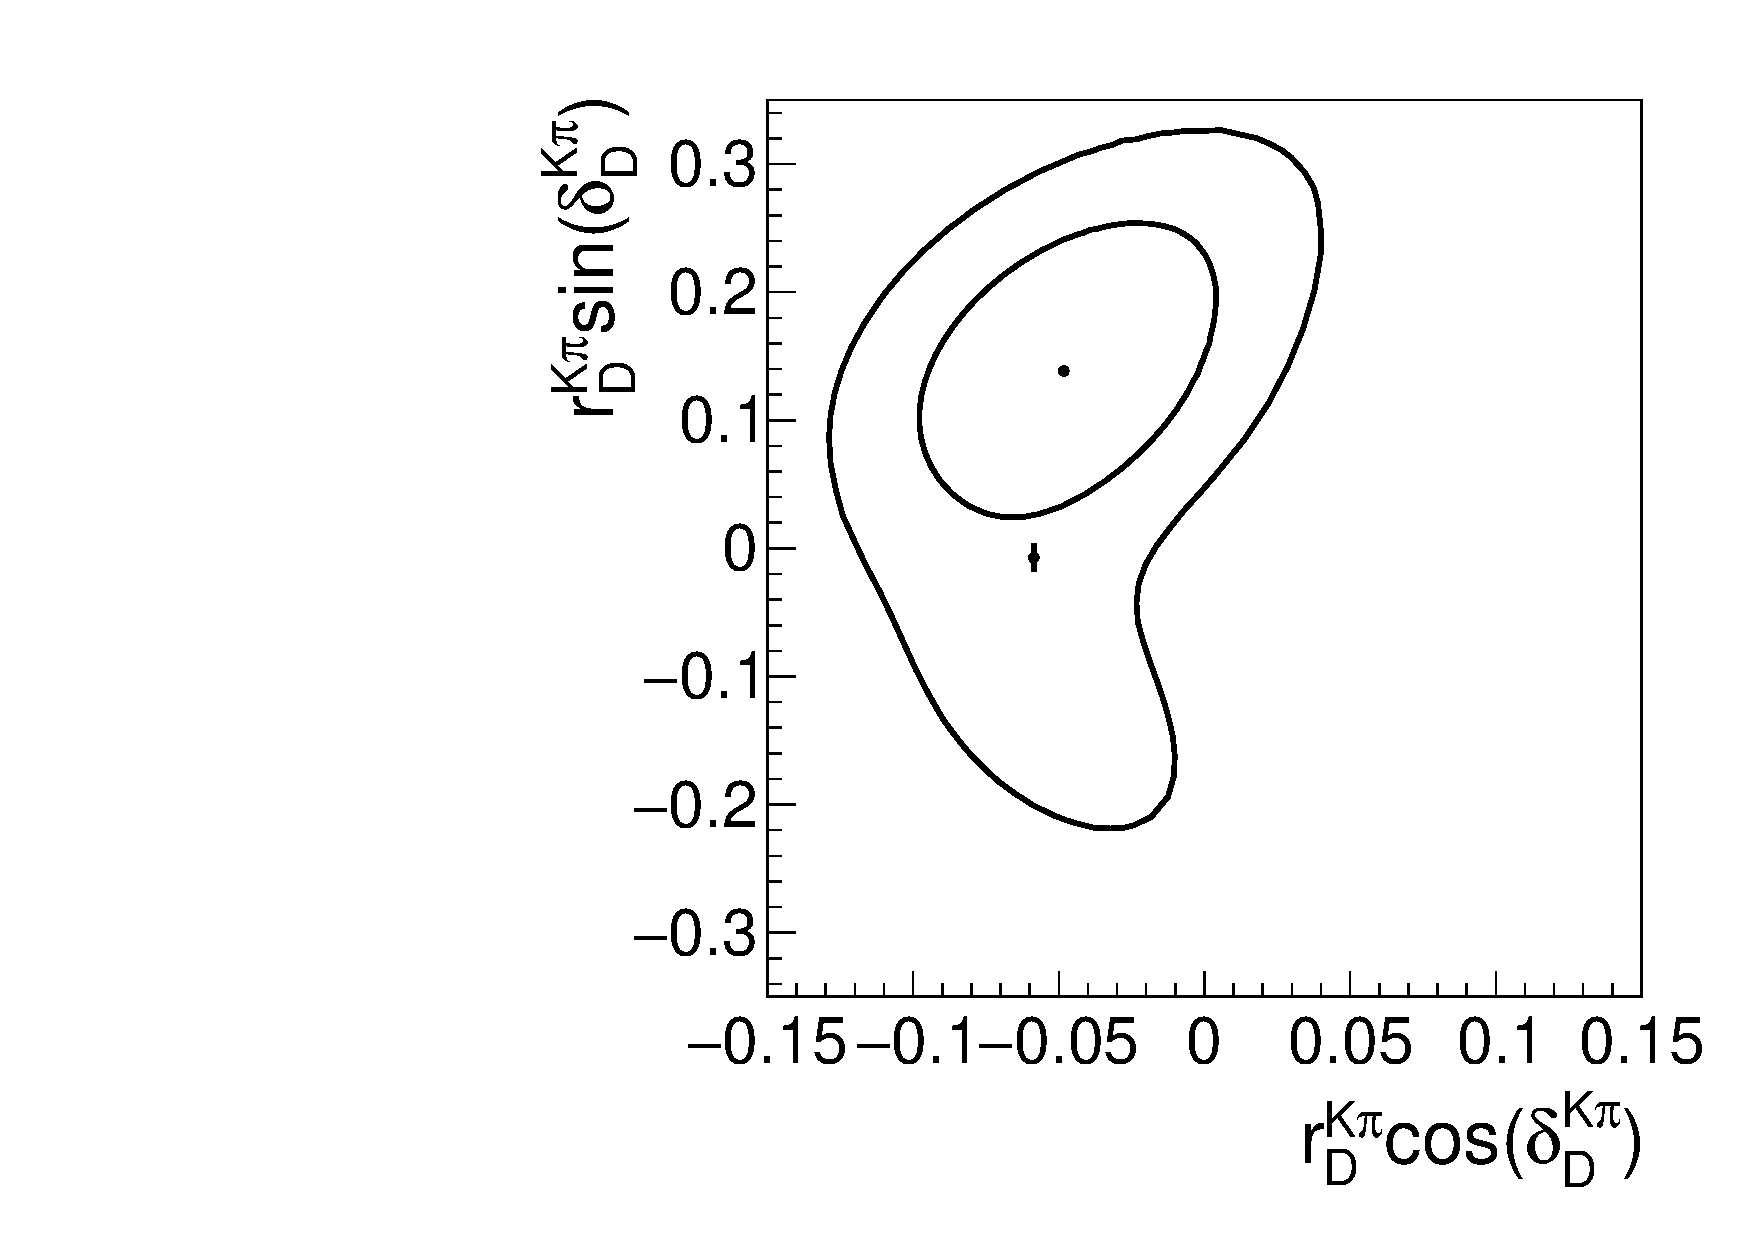
\includegraphics[width = 0.97\textwidth]{Plots/Contour_DeltaKpi_8invfb.pdf}
      \caption{$\SI{8}{\per\femto\barn}$}
    \end{subfigure}%
    \hspace{1cm}
    \begin{subfigure}{0.45\textwidth}
      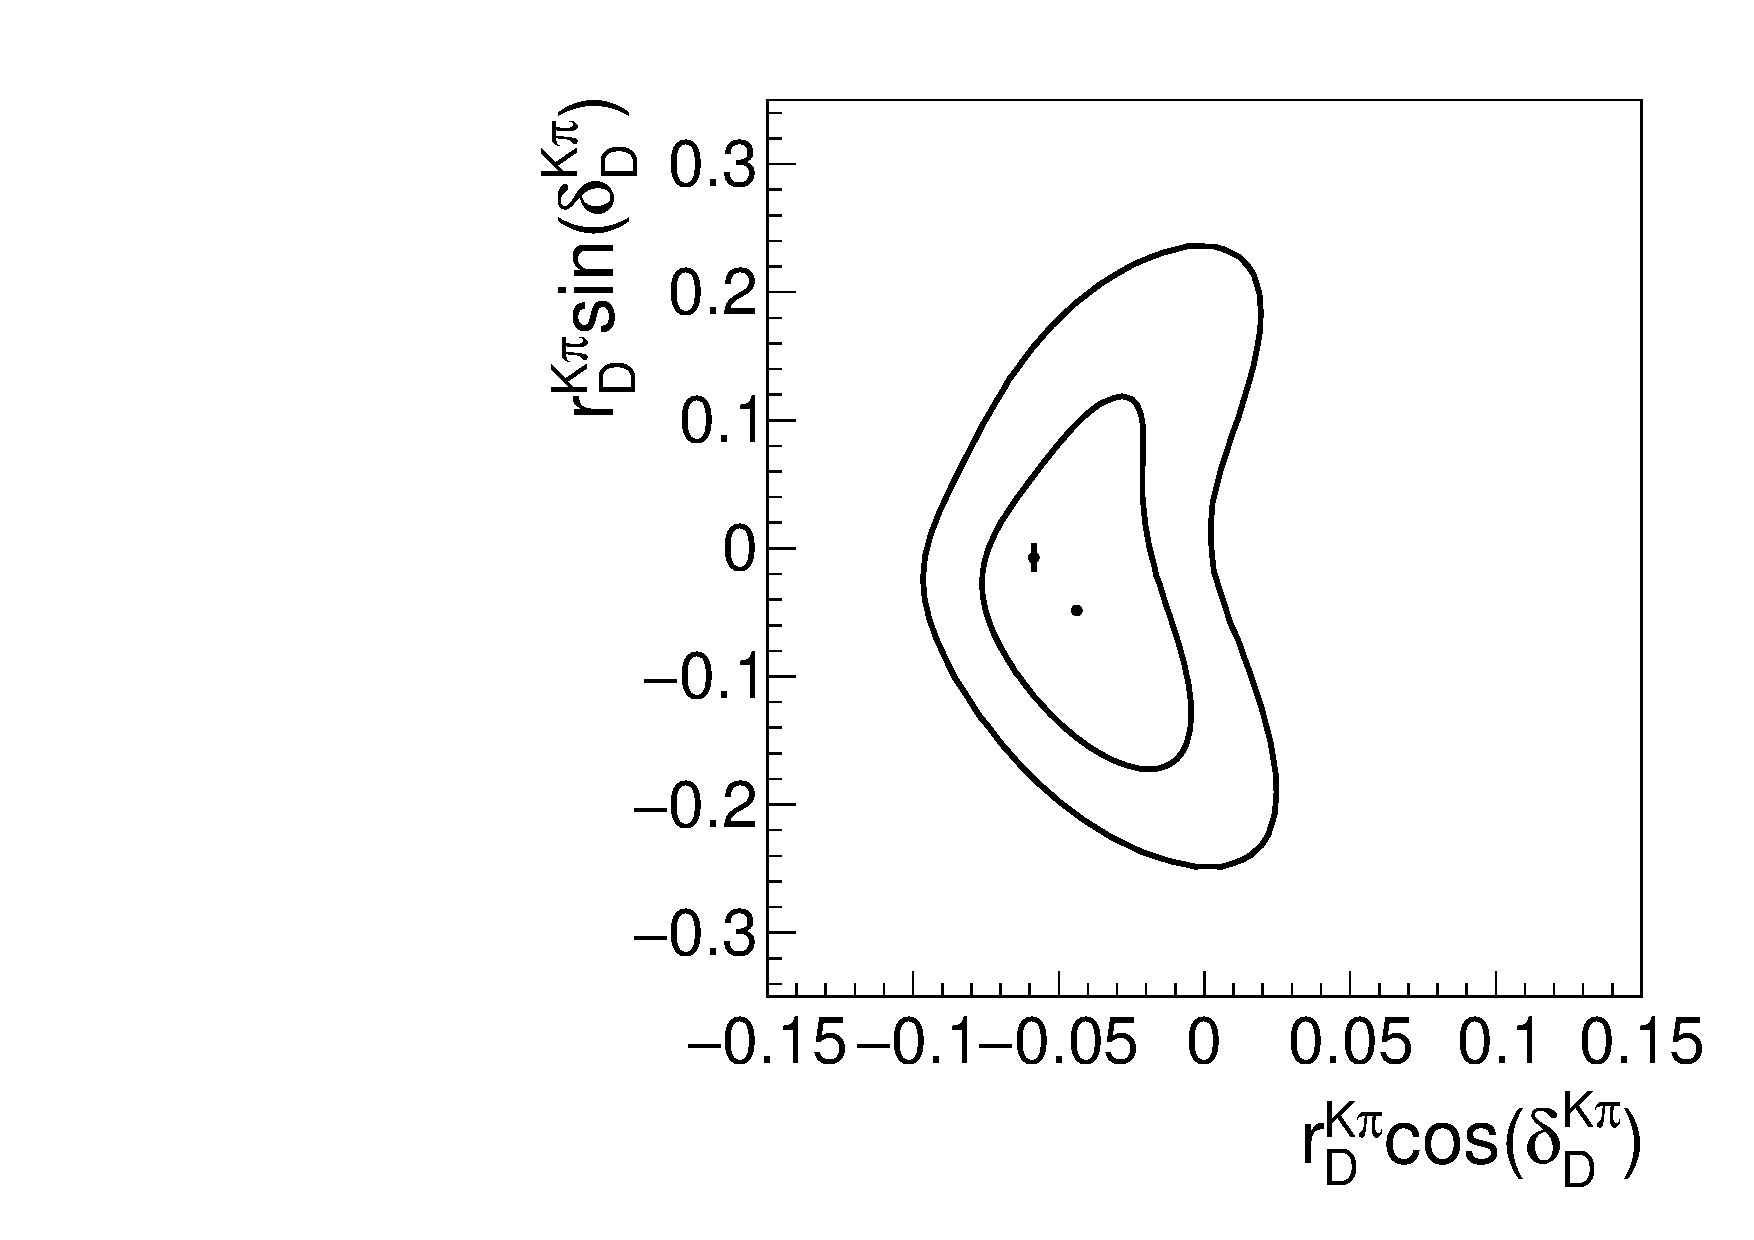
\includegraphics[width = 1.0\textwidth]{Plots/Contour_DeltaKpi_16invfb.pdf}
      \caption{$\SI{16}{\per\femto\barn}$}
    \end{subfigure}
    \caption{Warning: $r_D^{K\pi}\sin(\delta_D^{K\pi})$ uncertainties may be very non-Gaussian}
  \end{figure}
\end{frame}

\section{Summary and next steps}

\begin{frame}{Summary and next steps}
  \vspace{0.0cm}
  {\Large In summary:}
  \vspace{0.5cm}
  \begin{enumerate}
    \setlength\itemsep{1.0em}
    \item{BESIII analysis review is slowly moving forwards}
    \item{New data is available and preliminary results are very promising}
    \item{Aim to include new data without delaying the review process}
  \end{enumerate}
\end{frame}

\begin{frame}{Summary and next steps}
  \vspace{1.0cm}
  {\Large What now? The positive things first:}
  \vspace{0.5cm}
  \begin{itemize}
    \setlength\itemsep{1.0em}
    \item{Analysis for my thesis is more or less done}
    \item{Start preparation of $B^\pm\to[h^+h^-\pi^+\pi^-]_Dh^\pm$ for B2OC review}
    \item{Write thesis in parallel (perhaps this plan is too ambitious)}
  \end{itemize}
\end{frame}

\begin{frame}{Summary and next steps}
  \vspace{1.0cm}
  {\Large What now? The not so positive things last:}
  \vspace{0.5cm}
  \begin{itemize}
    \setlength\itemsep{1.0em}
    \item{Currently struggling with TORCH analysis...}
    \begin{enumerate}
      \item{Timing information is very challenging to interpret}
      \item{Calibrations are not finalised yet}
    \end{enumerate}
    \item{I haven't given up (yet), but I'm unsure about including TORCH chapter in my thesis}
  \end{itemize}
  \vspace{0.2cm}
  \begin{center}
    {\Large Thanks for your attention!}
  \end{center}
\end{frame}

\end{document}